%%%%%%%%%%%%%%%%%%%%%%%%%%%%%%%%%%%%%%%%
%%%%%  xPhO LaTeX Beamer Template  %%%%%
%%%%%  Date: 17/03/2025            %%%%%
%%%%%  Authors:                    %%%%%
%%%%%       Nguyen Thanh Long      %%%%%
%%%%%       Nguyen Le Mai Huong    %%%%%
%%%%%       Nguyen Minh Phuong     %%%%%
%%%%%%%%%%%%%%%%%%%%%%%%%%%%%%%%%%%%%%%%

\documentclass[aspectratio=169, t]{beamer} % Ratio 16:9
\usepackage[T5]{fontenc}
\usepackage{lmodern}
\usepackage{graphicx} 
\usepackage{array}
\usepackage{longtable} % for long table
\usepackage{chngcntr}
\counterwithin{figure}{section}
\usepackage{tcolorbox}
\renewcommand{\familydefault}{\sfdefault} % Font

\usepackage{caption}
\usepackage{siunitx}

\usepackage{tikz}
\usetikzlibrary{patterns}
\usepackage{subcaption}
\let\vec\relax
\newcommand{\vec}[1]{\textbf{#1}}

\usepackage{multicol}

\usepackage{mdframed}

% \definecolor{BlueDefault}{rgb}{0.2,0.2,0.7}
\definecolor{BlueDefault}{RGB}{14,47,95}


% Hide navigation 
\setbeamertemplate{navigation symbols}{}

% Setup background
\newcommand{\normalbackground}{%
    \usebackgroundtemplate{\includegraphics[width=\paperwidth,height=\paperheight]{Background/Normal_slide_xPhO.pdf}}%
}

\newcommand{\titlebackground}{%
    \usebackgroundtemplate{\includegraphics[width=\paperwidth,height=\paperheight]{Background/Title_slide_xPhO.pdf}}%
}

% Change the title color to white
\setbeamercolor{frametitle}{fg=white} 

% push the title up by \raisebox
\setbeamertemplate{frametitle}{%
    \vspace{0.3em}
    \hspace{-1em} \insertframetitle
    \vspace{2mm}
}

% Number of slide
\setbeamertemplate{footline}{%
    \hfill
    \insertframenumber/\inserttotalframenumber
    \hspace{7.5mm}
    \vspace{3.5mm}
}

%% Make Table of Contents %%
\AtBeginSection[]{
    \begin{frame}
        \frametitle{Mục lục}
        \begin{multicols}{2}
            \tableofcontents[currentsection]
        \end{multicols}
    \end{frame}
}

%% Section numbering %%
\setbeamertemplate{section in toc}[sections numbered]
\setbeamertemplate{subsection in toc}[subsections numbered]


\renewcommand{\figurename}{Hình}
\renewcommand{\tablename}{Bảng}

%%%%%%%%%% Pictures drawing %%%%%%%%%%%%%

\usepackage{pgfplots} %%%%%% Regression %%%%
\pgfplotsset{compat = newest}
\usepackage{pgfplotstable}
\usepackage{tikz}
\usepackage{tikz-3dplot} %%%%%% Draw %%%%%%
\usepackage{tikz,tkz-euclide}
\usetikzlibrary{arrows,calc,patterns}
\usetikzlibrary{quotes,angles}
\usetikzlibrary{shapes.geometric}
\usepackage{circuitikz} %%%%% Circuit %%%%
\usetikzlibrary{decorations.pathmorphing,patterns}


%%%%% Bibliography %%%%%
\usepackage[backend=biber,style=ieee]{biblatex}
\addbibresource{citation.bib}

\usepackage{url}
\usepackage{hyperref}
\hypersetup{
	colorlinks=true,
	linkcolor=BlueDefault,
	filecolor=BlueDefault,
    citecolor=BlueDefault,
	urlcolor=BlueDefault,
	pdftitle={Overleaf Example},
	pdfpagemode=FullScreen,
}

%%%%%%%%%% Color setup %%%%%%%%%%%%%

\RequirePackage{xcolor}
\definecolor{wsdred}{HTML}{8E1728}
\definecolor{wsdgrey}{HTML}{75787B}
\renewcommand{\normalcolor}{\color{wsdred}}
\colorlet{ColorOr}{white}

\begin{document}

\titlebackground

\begin{frame}[noframenumbering]
    \thispagestyle{empty}
    \bfseries
    \begin{flushleft}
        \vfill
        \vspace{5mm}
        \textcolor{BlueDefault}{\huge \bfseries ĐỘNG HỌC CHẤT ĐIỂM} \\
        \vspace{10mm}
        \textcolor{black}{\large \bfseries Người trình bày: Hirrus}
        \vfill
    \end{flushleft}
\end{frame}

\normalbackground

\begin{frame}{Giới thiệu chung}

Dao động là một quy luật lặp lại ở một mức độ nào đó. Chuyển động con lắc, chuyển động lò xo,... cũng là một loại dao động. Ta phân biệt dao động dựa trên bản chất vật lý của quá trình lặp lại đó: dao động cơ, dao động điện, dao động nhiệt,... 

\begin{center}
    \scalebox{0.8}{ 


% Pattern Info
 
\tikzset{
pattern size/.store in=\mcSize, 
pattern size = 5pt,
pattern thickness/.store in=\mcThickness, 
pattern thickness = 0.3pt,
pattern radius/.store in=\mcRadius, 
pattern radius = 1pt}
\makeatletter
\pgfutil@ifundefined{pgf@pattern@name@_dzn82le2u}{
\pgfdeclarepatternformonly[\mcThickness,\mcSize]{_dzn82le2u}
{\pgfqpoint{0pt}{0pt}}
{\pgfpoint{\mcSize+\mcThickness}{\mcSize+\mcThickness}}
{\pgfpoint{\mcSize}{\mcSize}}
{
\pgfsetcolor{\tikz@pattern@color}
\pgfsetlinewidth{\mcThickness}
\pgfpathmoveto{\pgfqpoint{0pt}{0pt}}
\pgfpathlineto{\pgfpoint{\mcSize+\mcThickness}{\mcSize+\mcThickness}}
\pgfusepath{stroke}
}}
\makeatother
\tikzset{every picture/.style={line width=0.75pt}} %set default line width to 0.75pt        

\begin{tikzpicture}[x=0.75pt,y=0.75pt,yscale=-1,xscale=1]
%uncomment if require: \path (0,14993); %set diagram left start at 0, and has height of 14993

%Shape: Resistor [id:dp0682999431650273] 
\draw   (708.36,14486.19) -- (705.65,14476.51) -- (699.18,14476) -- (709.7,14468.41) -- (696.77,14467.4) -- (707.28,14459.81) -- (694.35,14458.79) -- (704.87,14451.2) -- (691.94,14450.19) -- (702.45,14442.6) -- (695.99,14442.09) -- (693.28,14432.41) ;
%Straight Lines [id:da5213071163927143] 
\draw    (187.25,14453) -- (229.75,14560) ;
%Straight Lines [id:da7338233721265985] 
\draw    (174.5,14453) -- (200,14453) ;
%Shape: Rectangle [id:dp5191041423737714] 
\draw  [draw opacity=0][pattern=_dzn82le2u,pattern size=6pt,pattern thickness=0.75pt,pattern radius=0pt, pattern color={rgb, 255:red, 0; green, 0; blue, 0}] (200,14444) -- (174.5,14444) -- (174.5,14453) -- (200,14453) -- cycle ;
%Straight Lines [id:da12627081514921668] 
\draw  [dash pattern={on 4.5pt off 4.5pt}]  (187.25,14453) -- (187.25,14511) ;
%Shape: Arc [id:dp46541149684505223] 
\draw  [draw opacity=0] (202.65,14495.3) .. controls (197.92,14497.02) and (192.83,14497.97) .. (187.52,14498) -- (187.25,14453) -- cycle ; \draw   (202.65,14495.3) .. controls (197.92,14497.02) and (192.83,14497.97) .. (187.52,14498) ;  
%Shape: Circle [id:dp13890736711451002] 
\draw  [fill={rgb, 255:red, 0; green, 0; blue, 0 }  ,fill opacity=1 ] (219.25,14560) .. controls (219.25,14554.2) and (223.95,14549.5) .. (229.75,14549.5) .. controls (235.55,14549.5) and (240.25,14554.2) .. (240.25,14560) .. controls (240.25,14565.8) and (235.55,14570.5) .. (229.75,14570.5) .. controls (223.95,14570.5) and (219.25,14565.8) .. (219.25,14560) -- cycle ;
%Shape: Arc [id:dp4056604606124048] 
\draw  [draw opacity=0][dash pattern={on 0.84pt off 2.51pt}] (228.7,14560.54) .. controls (215.84,14565.5) and (201.86,14568.22) .. (187.25,14568.22) .. controls (174.91,14568.22) and (163.01,14566.28) .. (151.87,14562.68) -- (187.25,14453) -- cycle ; \draw  [dash pattern={on 0.84pt off 2.51pt}] (228.7,14560.54) .. controls (215.84,14565.5) and (201.86,14568.22) .. (187.25,14568.22) .. controls (174.91,14568.22) and (163.01,14566.28) .. (151.87,14562.68) ;  
%Straight Lines [id:da7220475113205878] 
\draw    (146.36,14560.92) -- (151.87,14562.68) ;
\draw [shift={(143.5,14560)}, rotate = 17.78] [fill={rgb, 255:red, 0; green, 0; blue, 0 }  ][line width=0.08]  [draw opacity=0] (8.93,-4.29) -- (0,0) -- (8.93,4.29) -- cycle    ;
%Shape: Resistor [id:dp4685865801258251] 
\draw   (708.4,14488.34) -- (718.64,14491.24) -- (722.13,14487.56) -- (724.24,14497.48) -- (731.23,14490.14) -- (733.34,14500.05) -- (740.33,14492.71) -- (742.45,14502.62) -- (749.44,14495.28) -- (751.55,14505.2) -- (755.04,14501.52) -- (765.28,14504.42) ;
%Shape: Ellipse [id:dp8924060191888339] 
\draw  [fill={rgb, 255:red, 0; green, 0; blue, 0 }  ,fill opacity=1 ] (699.84,14488.34) .. controls (699.84,14483.61) and (703.67,14479.78) .. (708.4,14479.78) .. controls (713.13,14479.78) and (716.96,14483.61) .. (716.96,14488.34) .. controls (716.96,14493.07) and (713.13,14496.9) .. (708.4,14496.9) .. controls (703.67,14496.9) and (699.84,14493.07) .. (699.84,14488.34) -- cycle ;
%Shape: Resistor [id:dp9517178099204282] 
\draw   (621.27,14504.42) -- (637.06,14501.25) -- (639.55,14495.47) -- (648.6,14504.22) -- (653.59,14492.66) -- (662.64,14501.41) -- (667.62,14489.85) -- (676.68,14498.59) -- (681.66,14487.04) -- (690.71,14495.78) -- (693.2,14490) -- (709,14486.84) ;
%Shape: Resistor [id:dp7529495263470161] 
\draw   (693.28,14576.42) -- (696.21,14560.48) -- (690.92,14555.84) -- (704.1,14550.94) -- (693.53,14541.67) -- (706.7,14536.76) -- (696.14,14527.49) -- (709.31,14522.59) -- (698.74,14513.32) -- (711.92,14508.42) -- (706.63,14503.78) -- (709.57,14487.84) ;
%Shape: Ellipse [id:dp7430715898296683] 
\draw  [dash pattern={on 1.69pt off 2.76pt}][line width=1.5]  (684.71,14504.42) .. controls (684.71,14499.69) and (688.55,14495.86) .. (693.28,14495.86) .. controls (698,14495.86) and (701.84,14499.69) .. (701.84,14504.42) .. controls (701.84,14509.14) and (698,14512.98) .. (693.28,14512.98) .. controls (688.55,14512.98) and (684.71,14509.14) .. (684.71,14504.42) -- cycle ;
%Shape: Capacitor [id:dp68096422209342] 
\draw   (497,14467) -- (497,14503) (517,14511) -- (477,14511) (517,14503) -- (477,14503) (497,14511) -- (497,14547) ;
%Shape: Inductor (Air Core) [id:dp4333840037799508] 
\draw   (362.82,14467) -- (362.82,14481.4) .. controls (368.6,14481.61) and (373.54,14483.61) .. (375.27,14486.43) .. controls (376.99,14489.26) and (375.16,14492.35) .. (370.64,14494.2) .. controls (367.11,14495.63) and (362.55,14496.21) .. (358.13,14495.8) .. controls (356.4,14495.8) and (355,14495.08) .. (355,14494.2) .. controls (355,14493.32) and (356.4,14492.6) .. (358.13,14492.6) .. controls (362.55,14492.19) and (367.11,14492.77) .. (370.64,14494.2) .. controls (374.39,14495.86) and (376.52,14498.18) .. (376.52,14500.6) .. controls (376.52,14503.02) and (374.39,14505.34) .. (370.64,14507) .. controls (367.11,14508.43) and (362.55,14509.01) .. (358.13,14508.6) .. controls (356.4,14508.6) and (355,14507.88) .. (355,14507) .. controls (355,14506.12) and (356.4,14505.4) .. (358.13,14505.4) .. controls (362.55,14504.99) and (367.11,14505.57) .. (370.64,14507) .. controls (374.39,14508.66) and (376.52,14510.98) .. (376.52,14513.4) .. controls (376.52,14515.82) and (374.39,14518.14) .. (370.64,14519.8) .. controls (367.11,14521.23) and (362.55,14521.81) .. (358.13,14521.4) .. controls (356.4,14521.4) and (355,14520.68) .. (355,14519.8) .. controls (355,14518.92) and (356.4,14518.2) .. (358.13,14518.2) .. controls (362.55,14517.79) and (367.11,14518.37) .. (370.64,14519.8) .. controls (375.16,14521.65) and (376.99,14524.74) .. (375.27,14527.57) .. controls (373.54,14530.39) and (368.6,14532.39) .. (362.82,14532.6) -- (362.82,14547) ;
%Straight Lines [id:da8285333313564818] 
\draw    (362.82,14547) -- (497,14547) ;
%Straight Lines [id:da624392190140687] 
\draw    (362.82,14467) -- (497,14467) ;

% Text Node
\draw (190,14498) node [anchor=north west][inner sep=0.75pt]    {$\varphi $};
% Text Node
\draw (334,14500) node [anchor=north west][inner sep=0.75pt]   [align=left] {L};
% Text Node
\draw (524,14500) node [anchor=north west][inner sep=0.75pt]   [align=left] {C};
% Text Node
\draw (147,14592) node [anchor=north west][inner sep=0.75pt]   [align=left] {(a) Dao động cơ};
\label{GT_dd cơ}
% Text Node
\draw (385,14592) node [anchor=north west][inner sep=0.75pt]   [align=left] {(b) Dao động điện};
\label{GT_dd điện}
% Text Node
\draw (631,14592) node [anchor=north west][inner sep=0.75pt]   [align=left] {(c) Dao động nhiệt};
\label{GT_dd nhiệt}


\end{tikzpicture} }
\end{center}



\end{frame}

\section{Phương trình vi phân}
\subsection{Số phức}
\begin{frame}{Số phức}
    \begin{center}
        \begin{minipage}{0.4\linewidth}
            \resizebox{1\linewidth}{!}{


\tikzset{every picture/.style={line width=0.75pt}} %set default line width to 0.75pt        

\begin{tikzpicture}[x=0.75pt,y=0.75pt,yscale=-1,xscale=1]
%uncomment if require: \path (0,15225); %set diagram left start at 0, and has height of 15225

%Straight Lines [id:da5015611160293443] 
\draw    (526,6086) -- (683.5,6086) ;
\draw [shift={(685.5,6086)}, rotate = 180] [color={rgb, 255:red, 0; green, 0; blue, 0 }  ][line width=0.75]    (10.93,-3.29) .. controls (6.95,-1.4) and (3.31,-0.3) .. (0,0) .. controls (3.31,0.3) and (6.95,1.4) .. (10.93,3.29)   ;
%Straight Lines [id:da7739785169188371] 
\draw    (526,6086) -- (526,5966) ;
\draw [shift={(526,5964)}, rotate = 90] [color={rgb, 255:red, 0; green, 0; blue, 0 }  ][line width=0.75]    (10.93,-3.29) .. controls (6.95,-1.4) and (3.31,-0.3) .. (0,0) .. controls (3.31,0.3) and (6.95,1.4) .. (10.93,3.29)   ;
%Straight Lines [id:da38078718023855684] 
\draw  [dash pattern={on 0.84pt off 2.51pt}]  (526,6033) -- (608.5,6033) ;
\draw [shift={(608.5,6033)}, rotate = 0] [color={rgb, 255:red, 0; green, 0; blue, 0 }  ][fill={rgb, 255:red, 0; green, 0; blue, 0 }  ][line width=0.75]      (0, 0) circle [x radius= 3.35, y radius= 3.35]   ;
%Straight Lines [id:da36972469805515473] 
\draw  [dash pattern={on 0.84pt off 2.51pt}]  (608.5,6033) -- (608.5,6086) ;

% Text Node
\draw (474,5948) node [anchor=north west][inner sep=0.75pt]    {$Im( z)$};
% Text Node
\draw (615,6008) node [anchor=north west][inner sep=0.75pt]    {$z\ =\ a\ +\ ib$};
% Text Node
\draw (682,6092) node [anchor=north west][inner sep=0.75pt]    {$Re( z)$};
% Text Node
\draw (601,6091) node [anchor=north west][inner sep=0.75pt]    {$a$};
% Text Node
\draw (505,6022) node [anchor=north west][inner sep=0.75pt]    {$b$};
% Text Node
\draw (507,6083) node [anchor=north west][inner sep=0.75pt]    {$O$};


\end{tikzpicture}}
        \end{minipage}
        \hspace{2mm}
        \begin{minipage}{0.4\linewidth}
            Số ảo \(\mathbf{i}\) được định nghĩa \cite{gilbert2009introduction}
            \begin{equation}
                i = \sqrt{-1}.
                \label{eq:1.1_1}
            \end{equation}
            Không gian số phức là 
            \begin{equation*}
                \mathcal{C} = (a,b) | a,b \in \mathcal{R}
            \end{equation*}
        \end{minipage}
    \end{center}
\end{frame}

\begin{frame}{Công thức euler}
    \begin{mdframed}[backgroundcolor=BlueDefault!10, linecolor=BlueDefault, linewidth=0.5pt, roundcorner=1pt]
        Công thức euler gọi là phép quay một góc \(\theta\) trong mặt phẳng phức.
        \begin{equation}
            e^{i\theta} = \cos{\theta} + i \sin{\theta}
            \label{eq:1.1_2}
        \end{equation}
    \end{mdframed}
    \vspace{2mm}
    
    Ví dụ: áp dụng phép quay \(\theta\) cho số phức \(z = a + i b\)
    \begin{center}
        \begin{minipage}{0.4\linewidth}
            \begin{equation*}
            \begin{split}
                \left[
            \begin{array}{c}
                a' \\
                b'
            \end{array}
            \right]  &= \left[\begin{array}{cc}
               \cos{\theta}  & -\sin{\theta} \\
               \sin{\theta}  & \cos{\theta}
            \end{array} \right] \left[
            \begin{array}{c}
                a \\
                b
            \end{array}
            \right]  \\
           z' &=  e^{i\theta}z
            \end{split}
            \end{equation*}
        \end{minipage}
        \hspace{1mm}
        \begin{minipage}{0.4\linewidth}
            \begin{center}
                \resizebox{1\linewidth}{!}{


\tikzset{every picture/.style={line width=0.75pt}} %set default line width to 0.75pt        

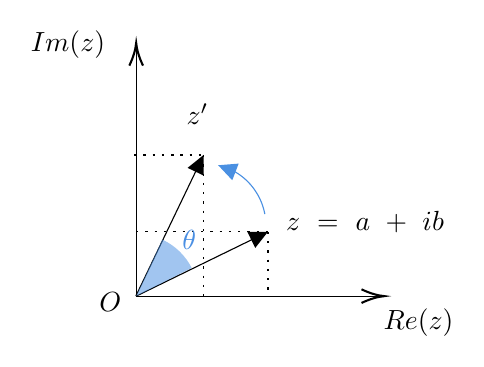
\begin{tikzpicture}[x=0.75pt,y=0.75pt,yscale=-1,xscale=1]
%uncomment if require: \path (0,15225); %set diagram left start at 0, and has height of 15225

%Straight Lines [id:da5015611160293443] 
\draw    (526,6086) -- (643.5,6086) ;
\draw [shift={(645.5,6086)}, rotate = 180] [color={rgb, 255:red, 0; green, 0; blue, 0 }  ][line width=0.75]    (10.93,-3.29) .. controls (6.95,-1.4) and (3.31,-0.3) .. (0,0) .. controls (3.31,0.3) and (6.95,1.4) .. (10.93,3.29)   ;
%Straight Lines [id:da7739785169188371] 
\draw    (526,6086) -- (526,5966) ;
\draw [shift={(526,5964)}, rotate = 90] [color={rgb, 255:red, 0; green, 0; blue, 0 }  ][line width=0.75]    (10.93,-3.29) .. controls (6.95,-1.4) and (3.31,-0.3) .. (0,0) .. controls (3.31,0.3) and (6.95,1.4) .. (10.93,3.29)   ;
%Straight Lines [id:da6097015977657645] 
\draw  [dash pattern={on 0.84pt off 2.51pt}]  (526,6055) -- (589.5,6055) ;
%Straight Lines [id:da06830863122513897] 
\draw  [dash pattern={on 0.84pt off 2.51pt}]  (589.5,6055) -- (589.5,6086) ;
%Straight Lines [id:da1339436079722769] 
\draw    (526,6086) -- (586.8,6056.32) ;
\draw [shift={(589.5,6055)}, rotate = 153.98] [fill={rgb, 255:red, 0; green, 0; blue, 0 }  ][line width=0.08]  [draw opacity=0] (8.93,-4.29) -- (0,0) -- (8.93,4.29) -- cycle    ;
%Straight Lines [id:da12876867450395124] 
\draw    (525.83,6086) -- (557.2,6020.7) ;
\draw [shift={(558.5,6018)}, rotate = 115.66] [fill={rgb, 255:red, 0; green, 0; blue, 0 }  ][line width=0.08]  [draw opacity=0] (8.93,-4.29) -- (0,0) -- (8.93,4.29) -- cycle    ;
%Straight Lines [id:da6964942743081263] 
\draw  [dash pattern={on 0.84pt off 2.51pt}]  (525,6018) -- (558.5,6018) ;
%Straight Lines [id:da21207065554446136] 
\draw  [dash pattern={on 0.84pt off 2.51pt}]  (558.5,6018) -- (558.5,6086) ;
%Straight Lines [id:da7448312272789616] 
\draw [color={rgb, 255:red, 74; green, 144; blue, 226 }  ,draw opacity=1 ]   (573.49,6026.01) -- (568.31,6024.02) ;
\draw [shift={(565.51,6022.94)}, rotate = 21.06] [fill={rgb, 255:red, 74; green, 144; blue, 226 }  ,fill opacity=1 ][line width=0.08]  [draw opacity=0] (8.93,-4.29) -- (0,0) -- (8.93,4.29) -- cycle    ;
%Shape: Arc [id:dp7227532122430883] 
\draw  [draw opacity=0] (573.49,6026.01) .. controls (580.94,6030.31) and (586.36,6037.72) .. (587.99,6046.47) -- (558.5,6052) -- cycle ; \draw  [color={rgb, 255:red, 74; green, 144; blue, 226 }  ,draw opacity=1 ] (573.49,6026.01) .. controls (580.94,6030.31) and (586.36,6037.72) .. (587.99,6046.47) ;  
%Shape: Arc [id:dp5675882433264926] 
\draw  [draw opacity=0][fill={rgb, 255:red, 74; green, 144; blue, 226 }  ,fill opacity=0.52 ] (538.61,6058.77) .. controls (544.71,6061.6) and (549.7,6066.42) .. (552.75,6072.4) -- (526,6086) -- cycle ; \draw  [draw opacity=0] (538.61,6058.77) .. controls (544.71,6061.6) and (549.7,6066.42) .. (552.75,6072.4) ;  

% Text Node
\draw (474,5957) node [anchor=north west][inner sep=0.75pt]    {$Im( z)$};
% Text Node
\draw (597,6044) node [anchor=north west][inner sep=0.75pt]    {$z\ =\ a\ +\ ib$};
% Text Node
\draw (644,6091) node [anchor=north west][inner sep=0.75pt]    {$Re( z)$};
% Text Node
\draw (507,6083) node [anchor=north west][inner sep=0.75pt]    {$O$};
% Text Node
\draw (549,5992) node [anchor=north west][inner sep=0.75pt]    {$z'$};
% Text Node
\draw (547,6053) node [anchor=north west][inner sep=0.75pt]    {$\textcolor[rgb]{0.29,0.56,0.89}{\theta }$};


\end{tikzpicture}}
            \end{center}
        \end{minipage}
    \end{center}
\end{frame}
\begin{frame}{Số phức}
    \begin{mdframed}[backgroundcolor=BlueDefault!10, linecolor=BlueDefault, linewidth=0.5pt, roundcorner=1pt]
        Công thức euler còn là cách biểu diễn khác của số phức.
        \begin{equation}
            z = |z| e^{i\theta} = |z|(\cos{\theta} + i \sin{\theta})
            \label{eq:1.1_3}
        \end{equation}
        Với \(|z|\) là module của số phức \(z\), \(\theta\) là góc lệch của so với trục thực.
    \end{mdframed}
    \begin{center}
        \begin{minipage}{0.4\linewidth}
        \resizebox{1\linewidth}{!}{


\tikzset{every picture/.style={line width=0.75pt}} %set default line width to 0.75pt        

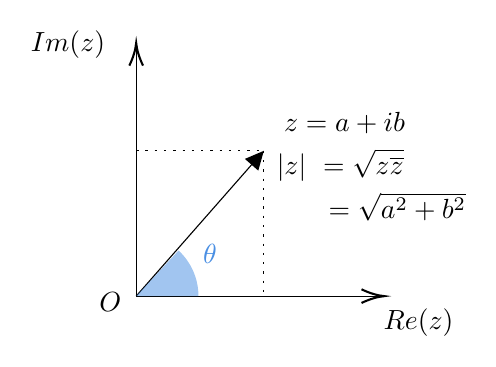
\begin{tikzpicture}[x=0.75pt,y=0.75pt,yscale=-1,xscale=1]
%uncomment if require: \path (0,15225); %set diagram left start at 0, and has height of 15225

%Straight Lines [id:da5597477618794069] 
\draw    (843,6091) -- (960.5,6091) ;
\draw [shift={(962.5,6091)}, rotate = 180] [color={rgb, 255:red, 0; green, 0; blue, 0 }  ][line width=0.75]    (10.93,-3.29) .. controls (6.95,-1.4) and (3.31,-0.3) .. (0,0) .. controls (3.31,0.3) and (6.95,1.4) .. (10.93,3.29)   ;
%Straight Lines [id:da12681955407125622] 
\draw    (843,6091) -- (843,5971) ;
\draw [shift={(843,5969)}, rotate = 90] [color={rgb, 255:red, 0; green, 0; blue, 0 }  ][line width=0.75]    (10.93,-3.29) .. controls (6.95,-1.4) and (3.31,-0.3) .. (0,0) .. controls (3.31,0.3) and (6.95,1.4) .. (10.93,3.29)   ;
%Straight Lines [id:da8100573273316289] 
\draw  [dash pattern={on 0.84pt off 2.51pt}]  (843,6021) -- (904.5,6021) ;
%Straight Lines [id:da18835817233889307] 
\draw  [dash pattern={on 0.84pt off 2.51pt}]  (904.5,6021) -- (904.5,6091) ;
%Straight Lines [id:da16390059449403382] 
\draw    (843,6091) -- (902.52,6023.25) ;
\draw [shift={(904.5,6021)}, rotate = 131.3] [fill={rgb, 255:red, 0; green, 0; blue, 0 }  ][line width=0.08]  [draw opacity=0] (8.93,-4.29) -- (0,0) -- (8.93,4.29) -- cycle    ;
%Shape: Arc [id:dp60111373870411] 
\draw  [draw opacity=0][fill={rgb, 255:red, 74; green, 144; blue, 226 }  ,fill opacity=0.52 ] (863.41,6069.02) .. controls (869.31,6074.49) and (873,6082.32) .. (873,6091) -- (843,6091) -- cycle ; \draw  [draw opacity=0] (863.41,6069.02) .. controls (869.31,6074.49) and (873,6082.32) .. (873,6091) ;  

% Text Node
\draw (791,5962) node [anchor=north west][inner sep=0.75pt]    {$Im( z)$};
% Text Node
\draw (913,6001) node [anchor=north west][inner sep=0.75pt]    {$z = a + ib$};
% Text Node
\draw (961,6096) node [anchor=north west][inner sep=0.75pt]    {$Re( z)$};
% Text Node
\draw (824,6088) node [anchor=north west][inner sep=0.75pt]    {$O$};
% Text Node
\draw (909.5,6019) node [anchor=north west][inner sep=0.75pt]    {$|z|\ =\sqrt{z \overline{z}}  $};
\draw (934.5,6040) node [anchor=north west][inner sep=0.75pt]    {$= \sqrt{a^2 + b^2} $};
% Text Node
\draw (874,6065) node [anchor=north west][inner sep=0.75pt]    {$\textcolor[rgb]{0.29,0.56,0.89}{\theta }$};


\end{tikzpicture}}
        \end{minipage}
        \hspace{3mm}
        \begin{minipage}{0.35\linewidth}
        Liên hợp phức: 
        \begin{equation}
            z = a + ib \rightarrow \overline{z} = a - ib.
            \label{eq:1.1_4}
        \end{equation}
        \end{minipage}
    \end{center}
\end{frame}
\subsection{Nguyên lý cộng dồn nghiệm}
\begin{frame}{PTVP tuyến tính}
    Phương trình vi phân tuyến tính là các phương trình chỉ bao gồm bậc nhất của các đạo hàm
    \begin{equation}
        \sum_{i=0}^n a_i x ^{(i)} = C.
        \label{eq:1.2_1}
    \end{equation}
    Khi chúng ta giải ra các nghiệm \((x_1, x_2,..., x_n)\) thoả mãn phương trình vi phân tuyến tính. Thì ta nói, nghiệm tổng quát là tổ hợp tuyến tính của các nghiệm
    \begin{equation}
        x_{tq} = A_1 x_1 + A_2 + ... + A_n x_n.
        \label{eq:1.2_2}
    \end{equation}
\end{frame}
\begin{frame}{Cộng dồn nghiệm}
\begin{center}
        \resizebox{0.6\linewidth}{!}{


\tikzset{every picture/.style={line width=0.75pt}} %set default line width to 0.75pt        

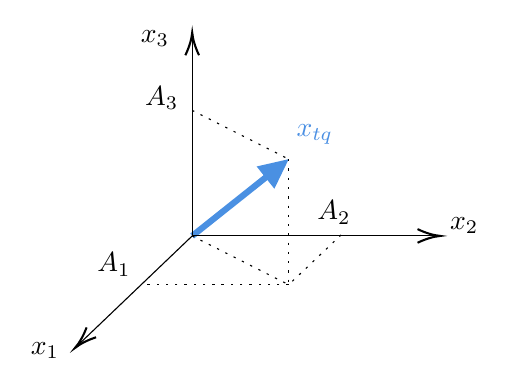
\begin{tikzpicture}[x=0.75pt,y=0.75pt,yscale=-1,xscale=1]
%uncomment if require: \path (0,15225); %set diagram left start at 0, and has height of 15225

%Straight Lines [id:da21513560769145257] 
\draw [color={rgb, 255:red, 74; green, 144; blue, 226 }  ,draw opacity=1 ][line width=2.25]    (204,5975) -- (246.59,5941.11) ;
\draw [shift={(250.5,5938)}, rotate = 141.49] [fill={rgb, 255:red, 74; green, 144; blue, 226 }  ,fill opacity=1 ][line width=0.08]  [draw opacity=0] (14.29,-6.86) -- (0,0) -- (14.29,6.86) -- cycle    ;
%Straight Lines [id:da8820661847854037] 
\draw    (204,5975) -- (321.5,5975) ;
\draw [shift={(323.5,5975)}, rotate = 180] [color={rgb, 255:red, 0; green, 0; blue, 0 }  ][line width=0.75]    (10.93,-3.29) .. controls (6.95,-1.4) and (3.31,-0.3) .. (0,0) .. controls (3.31,0.3) and (6.95,1.4) .. (10.93,3.29)   ;
%Straight Lines [id:da5315178017564863] 
\draw    (204,5975) -- (148.95,6027.62) ;
\draw [shift={(147.5,6029)}, rotate = 316.3] [color={rgb, 255:red, 0; green, 0; blue, 0 }  ][line width=0.75]    (10.93,-3.29) .. controls (6.95,-1.4) and (3.31,-0.3) .. (0,0) .. controls (3.31,0.3) and (6.95,1.4) .. (10.93,3.29)   ;
%Straight Lines [id:da14510782407127987] 
\draw    (204,5975) -- (204,5879) ;
\draw [shift={(204,5877)}, rotate = 90] [color={rgb, 255:red, 0; green, 0; blue, 0 }  ][line width=0.75]    (10.93,-3.29) .. controls (6.95,-1.4) and (3.31,-0.3) .. (0,0) .. controls (3.31,0.3) and (6.95,1.4) .. (10.93,3.29)   ;
%Straight Lines [id:da982507304256855] 
\draw  [dash pattern={on 0.84pt off 2.51pt}]  (250.5,5938) -- (250.5,5998.5) ;
%Straight Lines [id:da6681397441647374] 
\draw  [dash pattern={on 0.84pt off 2.51pt}]  (250.5,5998.5) -- (179.5,5998.5) ;
%Straight Lines [id:da7275191331520965] 
\draw  [dash pattern={on 0.84pt off 2.51pt}]  (204,5914.5) -- (250.5,5938) ;
%Straight Lines [id:da6882271778151009] 
\draw  [dash pattern={on 0.84pt off 2.51pt}]  (275.75,5974.5) -- (250.5,5998.5) ;
%Straight Lines [id:da4278104229055373] 
\draw  [dash pattern={on 0.84pt off 2.51pt}]  (204,5975) -- (250.5,5998.5) ;

% Text Node
\draw (253,5920) node [anchor=north west][inner sep=0.75pt]    {$\textcolor[rgb]{0.29,0.56,0.89}{x_{tq}}$};
% Text Node
\draw (125,6025) node [anchor=north west][inner sep=0.75pt]    {$x_{1}$};
% Text Node
\draw (327,5965) node [anchor=north west][inner sep=0.75pt]    {$x_{2}$};
% Text Node
\draw (178,5875) node [anchor=north west][inner sep=0.75pt]    {$x_{3}$};
% Text Node
\draw (157,5982) node [anchor=north west][inner sep=0.75pt]    {$A _{1}$};
% Text Node
\draw (263,5957) node [anchor=north west][inner sep=0.75pt]    {$A _{2}$};
% Text Node
\draw (180,5902) node [anchor=north west][inner sep=0.75pt]    {$A _{3}$};


\end{tikzpicture}}
\end{center}
\end{frame}
\subsection{PTVP bậc 2 thuần nhất}
\begin{frame}{PTVP bậc 2 thuần nhất}
    Ta gọi một PTVP là bậc 2  thuần nhất khi nó có dạng \cite{morin2008introduction}
    \begin{equation}
        a_0 x + a_1 x' + a_2 x'' = 0.
        \label{eq:1.3_1}
    \end{equation}
    Ta giả sử \(x\) có dạng \(x = A e^{\lambda t}\). Ta thế vào phương trình \ref{eq:1.3_1}. 
    \begin{equation*}
    \begin{split}
        & A e^{\lambda t} ( a_0 + a_1 \lambda + a_2 \lambda_2) = 0
        \\
       \Rightarrow \ & a_2 \lambda^2 + a_1 \lambda + a_0 = 0.
    \end{split}
    \end{equation*}
    Ta gọi phương trình đa thức bậc 2 ở trên là "phương trình đặc trưng". 
    \begin{equation*}
        \Delta = a_1^2 - 4 a_0 a_2.
    \end{equation*}
\end{frame}

\begin{frame}{Các trường hợp}
    \textbf{Trường hợp 1:} \(\Delta < 0\)
    \vspace{2mm}

    Khi này, nghiệm \(\lambda\) sẽ có dạng
    \begin{equation*}
    \displaystyle 
        \lambda_{1,2} = -\frac{a_1 \pm i \sqrt{4 a_0 a_2 - a_1^2}}{2a_2} \equiv \alpha \pm i \beta.
    \end{equation*}
    Các nghiệm của PTVP lần lượt là
    \begin{equation*}
        x_1 =  e^{\lambda_1 t}; \ x_2 =  e^{\lambda_2 t}.
    \end{equation*}
    Nghiệm tổng quát
    \begin{equation*}
    \begin{split}
        x_{tq} &= A_1 e^{\lambda_1 t} + A_2 e^{\lambda_2 t} \\
        &= e^{\alpha t} \left( A_1 e^{i\beta t} + A_2 e^{-i\beta t} \right).
    \end{split}
    \end{equation*}
\end{frame}
\begin{frame}{Các trường hợp}
    Do \(x_{tq}\) là hàm thực, nên ta có những điều kiện sau
    \begin{equation*}
    \left\{
    \begin{array}{ccc}
    A_1 + A_2 &=& C \cos \phi \\
    A_1 - A_2 &=& i C \sin \phi
    \end{array}
    \right.
    \end{equation*}
    Dựa vào công thức euler, ta sẽ thu được
    \begin{equation*}
        x_{tq} = C e^{\alpha t} \cos{(\beta t + \varphi)}.
    \end{equation*}
\end{frame}
\begin{frame}{Các trường hợp}
    \textbf{Trường hợp 2:} \(\Delta > 0\)
    \vspace{2mm}

    Khi này, nghiệm \(\lambda\) sẽ có dạng
    \begin{equation*}
        \lambda_{1,2} = -\frac{a_1 \pm  \sqrt{a_1^2-4 a_2 a_0}}{2a_2}.
    \end{equation*}
    Các nghiệm của PTVP lần lượt là
    \begin{equation*}
        x_1 = e^{\lambda_1 t} ; \ x_2 = e^{\lambda_2 t}.
    \end{equation*}
    Nghiệm tổng quát
    \begin{equation*}
        x_{tq} = A_1 e^{\lambda_1 t} + A_2e^{\lambda_2 t}.
    \end{equation*}
\end{frame}
\begin{frame}{Các trường hợp}
    \textbf{Trường hợp 3:} \(\Delta =0\)
    \vspace{2mm}

    Khi này, nghiệm \(\lambda\) sẽ có dạng
    \begin{equation*}
        \lambda = -\frac{a_1}{2a_2}.
    \end{equation*}

    Các nghiệm của PTVP lần lượt là 
    \begin{equation*}
        x_1 = e^{\lambda t}; \ x_2 = t e^{\lambda t}.
    \end{equation*}
    Nghiệm tổng quát
    \begin{equation*}
    \begin{split}
        x_{tq} &= A_1 e^{\lambda t} + A_2 t e^{\lambda t} \\
        &=e^{\lambda t} (A_1 + A_2 t).
    \end{split}
    \end{equation*}
\end{frame}
\begin{frame}{Tổng kết}
    \begin{equation*}
        \begin{array}{|l|c|}
        \hline
        \text{Trường hợp} & \text{Nghiệm} \\ 
        \hline
        \begin{array}{l}
        \Delta < 0 \\
        \lambda = a + ib
        \end{array}
        & x = C e^{-at} \cos(bt + \varphi) \\
        \hline
        \begin{array}{l}
        \Delta > 0 \\
        \lambda = \lambda_{1,2}
        \end{array}
        & x = Ae^{\lambda_1 t} + B e^{\lambda_2 t} \\
        \hline
        \begin{array}{l}
        \Delta = 0 \\
        \lambda = a
        \end{array}
        & x = e^{at} (A + Bt) \\
        \hline
        \end{array}
    \end{equation*}
\end{frame}
\subsection{PTVP bậc 2 không thuần nhất}
\begin{frame}{PTVP bậc 2 không thuần nhất}
    Phương trình vi phân bậc 2 không thuần có dạng
    \begin{equation}
        a_0 x + a_1 x' + a_2 x'' = f(t)
        \label{eq:1.4_1}
    \end{equation}
    Nghiệm tổng quát \(x_{tq}\) có dạng
    \begin{equation*}
        x_{tq} = x_{tn} + x_{r}
    \end{equation*}
    Khi thế vào phương trình (\ref{eq:1.4_1}).
    \begin{equation*}
        (a_0 x_{tn} + a_1 x_{tn}' + a_2 x_{tn}'') + (a_0 x_r + a_1 x_r' + a_2 x_r'') = 0 + f(t).
    \end{equation*}
\end{frame}
\begin{frame}{Giải nghiệm riêng}
    \(x_r\) tuân theo đặc trưng của \(f(t)\).
    \begin{enumerate}[\textbullet]
        \item Nếu \(f(t)\) là đa thức bậc n \(\rightarrow\) x cũng có dạng đa thức bậc n.
        \item Nếu \(f(t)\) là hàm \(\cos{()}\) \(\rightarrow\) x cũng có dạng \(A_r \cos{()} + B_r \sin{()}\).
    \end{enumerate}
    \textbf{!!!} Phải tìm những hệ số.
    \vspace{2mm}
    \pause

    Ví dụ: tìm nghiệm riêng của \(a_0 x + a_1 x' + a_2 x'' = \alpha x^2 + \beta x + \gamma\)
    \pause
    \vspace{2mm}

    \begin{center}
        \begin{minipage}{0.45\linewidth}
        \underline{Giải}
        \vspace{2mm}
        
            Giả sử \(x_r = A x^2 + B x + C\), thế vô PTVP ta sẽ có dạng
            \begin{equation*}
                ()x^2 + ()x + () = \alpha x^2 + \beta x + \gamma
            \end{equation*}
        \end{minipage}
        \hspace{3mm}
        \begin{minipage}{0.45\linewidth}
            Đồng nhất hai vế
            \begin{equation*}
            \left\{
                \begin{array}{lcl}
                a_0 A &=& \alpha \\
                2a_1 A + a_0 B &=& \beta \\
                2a_2 A + a_1 B + a_0 C &=& \gamma
                \end{array}
            \right.
            \end{equation*}
        \end{minipage}
    \end{center}
    
    
\end{frame}


\section{Dao động một chất điểm}

\subsection{Dao động điều hoà}
\begin{frame}{Phương trình dao động điều hoà}
    Phương trình dao động điều hoà
    \begin{equation}
        x = A \cos{(\omega t +\varphi)}
    \end{equation}
    \vspace{5mm}
    
    \begin{center}
        \resizebox{0.7\linewidth}{!}{


% Pattern Info
 
\tikzset{
pattern size/.store in=\mcSize, 
pattern size = 5pt,
pattern thickness/.store in=\mcThickness, 
pattern thickness = 0.3pt,
pattern radius/.store in=\mcRadius, 
pattern radius = 1pt}
\makeatletter
\pgfutil@ifundefined{pgf@pattern@name@_bjzsyyhfx}{
\pgfdeclarepatternformonly[\mcThickness,\mcSize]{_bjzsyyhfx}
{\pgfqpoint{0pt}{0pt}}
{\pgfpoint{\mcSize+\mcThickness}{\mcSize+\mcThickness}}
{\pgfpoint{\mcSize}{\mcSize}}
{
\pgfsetcolor{\tikz@pattern@color}
\pgfsetlinewidth{\mcThickness}
\pgfpathmoveto{\pgfqpoint{0pt}{0pt}}
\pgfpathlineto{\pgfpoint{\mcSize+\mcThickness}{\mcSize+\mcThickness}}
\pgfusepath{stroke}
}}
\makeatother
\tikzset{every picture/.style={line width=0.75pt}} %set default line width to 0.75pt        

\begin{tikzpicture}[x=0.75pt,y=0.75pt,yscale=-1,xscale=1]
%uncomment if require: \path (0,15225); %set diagram left start at 0, and has height of 15225

%Straight Lines [id:da437877768560178] 
\draw    (129,6269) -- (129,6301) ;
%Straight Lines [id:da3724100858381515] 
\draw    (473.5,6301) -- (129,6301) ;
%Shape: Rectangle [id:dp7198122251048675] 
\draw  [draw opacity=0][pattern=_bjzsyyhfx,pattern size=6pt,pattern thickness=0.75pt,pattern radius=0pt, pattern color={rgb, 255:red, 0; green, 0; blue, 0}] (129,6269) -- (103.5,6269) -- (103.5,6301) -- (129,6301) -- cycle ;
%Shape: Resistor [id:dp36636194347067563] 
\draw   (129,6285) -- (145.65,6285) -- (149.35,6276.13) -- (156.75,6293.88) -- (164.15,6276.13) -- (171.55,6293.88) -- (178.95,6276.13) -- (186.35,6293.88) -- (193.75,6276.13) -- (201.15,6293.88) -- (204.85,6285) -- (221.5,6285) ;
%Shape: Square [id:dp9363148260133486] 
\draw   (221.5,6269) -- (253.5,6269) -- (253.5,6301) -- (221.5,6301) -- cycle ;
%Shape: Square [id:dp6956049205778242] 
\draw  [dash pattern={on 0.84pt off 2.51pt}] (266.5,6269) -- (298.5,6269) -- (298.5,6301) -- (266.5,6301) -- cycle ;
%Straight Lines [id:da8946582938824832] 
\draw    (470.5,6332) -- (282.5,6332) ;
\draw [shift={(282.5,6332)}, rotate = 360] [color={rgb, 255:red, 0; green, 0; blue, 0 }  ][line width=0.75]    (0,5.59) -- (0,-5.59)   ;
\draw [shift={(473.5,6332)}, rotate = 180] [fill={rgb, 255:red, 0; green, 0; blue, 0 }  ][line width=0.08]  [draw opacity=0] (8.93,-4.29) -- (0,0) -- (8.93,4.29) -- cycle    ;
%Straight Lines [id:da3156418836856203] 
\draw    (282.5,6332) -- (121.5,6332) ;
%Straight Lines [id:da3718838593743382] 
\draw    (244.5,6254) -- (287,6254) ;
\draw [shift={(241.5,6254)}, rotate = 0] [fill={rgb, 255:red, 0; green, 0; blue, 0 }  ][line width=0.08]  [draw opacity=0] (8.93,-4.29) -- (0,0) -- (8.93,4.29) -- cycle    ;
%Straight Lines [id:da06935968887205124] 
\draw    (185.5,6332) -- (282.5,6332) ;
\draw [shift={(185.5,6332)}, rotate = 180] [color={rgb, 255:red, 0; green, 0; blue, 0 }  ][line width=0.75]    (0,5.59) -- (0,-5.59)   ;
%Straight Lines [id:da7035616424166616] 
\draw    (282.5,6332) -- (379.5,6332) ;
\draw [shift={(379.5,6332)}, rotate = 180] [color={rgb, 255:red, 0; green, 0; blue, 0 }  ][line width=0.75]    (0,5.59) -- (0,-5.59)   ;

% Text Node
\draw (166,6251) node [anchor=north west][inner sep=0.75pt]   [align=left] {k};
% Text Node
\draw (469.5,6338) node [anchor=north west][inner sep=0.75pt]   [align=left] {x};
% Text Node
\draw (237.5,6285) node   [align=left] {m};
% Text Node
\draw (282.5,6340) node [anchor=north] [inner sep=0.75pt]   [align=left] {O};
% Text Node
\draw (258,6230) node [anchor=north west][inner sep=0.75pt]   [align=left] {x};
% Text Node
\draw (380,6340) node [anchor=north] [inner sep=0.75pt]   [align=left] {A};
% Text Node
\draw (180,6340) node [anchor=north] [inner sep=0.75pt]   [align=left] {\mbox{-} A};


\end{tikzpicture}}
    \end{center}
\end{frame}

\begin{frame}{Hệ dao động điều hoà - PTVP}
    \begin{center}
        


% Pattern Info
 
\tikzset{
pattern size/.store in=\mcSize, 
pattern size = 5pt,
pattern thickness/.store in=\mcThickness, 
pattern thickness = 0.3pt,
pattern radius/.store in=\mcRadius, 
pattern radius = 1pt}
\makeatletter
\pgfutil@ifundefined{pgf@pattern@name@_sq81xq6mf}{
\pgfdeclarepatternformonly[\mcThickness,\mcSize]{_sq81xq6mf}
{\pgfqpoint{0pt}{0pt}}
{\pgfpoint{\mcSize+\mcThickness}{\mcSize+\mcThickness}}
{\pgfpoint{\mcSize}{\mcSize}}
{
\pgfsetcolor{\tikz@pattern@color}
\pgfsetlinewidth{\mcThickness}
\pgfpathmoveto{\pgfqpoint{0pt}{0pt}}
\pgfpathlineto{\pgfpoint{\mcSize+\mcThickness}{\mcSize+\mcThickness}}
\pgfusepath{stroke}
}}
\makeatother
\tikzset{every picture/.style={line width=0.75pt}} %set default line width to 0.75pt        

\begin{tikzpicture}[x=0.75pt,y=0.75pt,yscale=-1,xscale=1]
%uncomment if require: \path (0,15225); %set diagram left start at 0, and has height of 15225

%Straight Lines [id:da857908311406453] 
\draw    (393.5,14972) -- (394,15057) ;
%Straight Lines [id:da29061278759721887] 
\draw    (619.5,15057) -- (394,15057) ;
%Shape: Rectangle [id:dp9455351102890761] 
\draw  [draw opacity=0][pattern=_sq81xq6mf,pattern size=6pt,pattern thickness=0.75pt,pattern radius=0pt, pattern color={rgb, 255:red, 0; green, 0; blue, 0}] (393.5,14972) -- (368.5,14972) -- (368.5,15057) -- (393.5,15057) -- cycle ;
%Shape: Resistor [id:dp1655417168724569] 
\draw   (393.75,15014.5) -- (410.4,15014.5) -- (414.1,15005.63) -- (421.5,15023.38) -- (428.9,15005.63) -- (436.3,15023.38) -- (443.7,15005.63) -- (451.1,15023.38) -- (458.5,15005.63) -- (465.9,15023.38) -- (469.6,15014.5) -- (486.25,15014.5) ;
%Shape: Square [id:dp5547088787123857] 
\draw   (486.5,14972) -- (571.5,14972) -- (571.5,15057) -- (486.5,15057) -- cycle ;
%Straight Lines [id:da9821701492442481] 
\draw    (638.5,15087) -- (532.5,15087) ;
\draw [shift={(532.5,15087)}, rotate = 360] [color={rgb, 255:red, 0; green, 0; blue, 0 }  ][line width=0.75]    (0,5.59) -- (0,-5.59)   ;
\draw [shift={(641.5,15087)}, rotate = 180] [fill={rgb, 255:red, 0; green, 0; blue, 0 }  ][line width=0.08]  [draw opacity=0] (8.93,-4.29) -- (0,0) -- (8.93,4.29) -- cycle    ;
%Straight Lines [id:da4621297135617979] 
\draw    (532.5,15087) -- (423.5,15087) ;

% Text Node
\draw (435,14980) node [anchor=north west][inner sep=0.75pt]   [align=left] {k};
% Text Node
\draw (641.5,15087) node [anchor=north west][inner sep=0.75pt]   [align=left] {x};
% Text Node
\draw (529,15014.5) node   [align=left] {M};
% Text Node
\draw (532.5,15095) node [anchor=north] [inner sep=0.75pt]   [align=left] {O};


\end{tikzpicture}
    \end{center}
    Tổng lực tác động lên vật (lúc này chỉ gồm lực lò xo)
    \begin{equation*}
        \mathbf{F} = - k \mathbf{x}.
    \end{equation*}
    \pause
    Bản chất là đi giải phương trình vi phân:
    \begin{equation}
        m x'' = - k x.
    \end{equation}
\end{frame}

\subsection{Dao động điều hoà có cản}
\subsubsection{Dao động có cản khô}
\begin{frame}{Hệ DĐ có cản khô}
    \begin{center}
        \resizebox{1\linewidth}{!}{\input{Content/Image/2.2_1}}
    \end{center}
    Lúc này hệ chịu thêm một lực ma sát khô. Tổng lực tác động lên vật

\end{frame}
\begin{frame}{Hệ DĐ có cản khô - PTVP}
    Lúc này ta giải cùng lúc hai phương trình vi phân
    \begin{equation}
    \left\{
        \begin{split}
            m x'' &= -kx + \mu N \\
            m x'' &= -kx - \mu N
        \end{split}
    \right.
    \end{equation}
    Đặt \(a=x-\mu N/k\) và \(b=x+\mu N/k\) ta có.
    \begin{equation}
    \left\{
        \begin{split}
        a'' + \omega^2 a &= 0 \\
        b'' + \omega^2 b &= 0
        \end{split}
    \right.
    \end{equation}
    Ta có hai nghiệm:
    \begin{equation}
    \left\{
        \begin{array}{ccc}
        a &=&\displaystyle x -\frac{\mu N}{k} = A \cos{(\omega t + \varphi_a)} 
        \\
        \\
        b &=&\displaystyle x +\frac{\mu N}{k} = B \cos{(\omega t + \varphi_b)}
        \end{array}
    \right.
    \end{equation}
\end{frame}

\begin{frame}{Hệ DĐ có cản khô - PTVP}
    Nghiệm \(a\) ứng với trường hợp vật đang đi cùng chiều dương. Nghiệm \(b\) ứng với trường hợp vật đang đi ngược chiều dương. 
    \vspace{2mm}

    Trường hợp vật đi giống nghiệm \(a\)
    \vspace{5mm}
    
    \begin{center}
        


% Pattern Info
 
\tikzset{
pattern size/.store in=\mcSize, 
pattern size = 5pt,
pattern thickness/.store in=\mcThickness, 
pattern thickness = 0.3pt,
pattern radius/.store in=\mcRadius, 
pattern radius = 1pt}
\makeatletter
\pgfutil@ifundefined{pgf@pattern@name@_lh2po6njo}{
\pgfdeclarepatternformonly[\mcThickness,\mcSize]{_lh2po6njo}
{\pgfqpoint{0pt}{0pt}}
{\pgfpoint{\mcSize+\mcThickness}{\mcSize+\mcThickness}}
{\pgfpoint{\mcSize}{\mcSize}}
{
\pgfsetcolor{\tikz@pattern@color}
\pgfsetlinewidth{\mcThickness}
\pgfpathmoveto{\pgfqpoint{0pt}{0pt}}
\pgfpathlineto{\pgfpoint{\mcSize+\mcThickness}{\mcSize+\mcThickness}}
\pgfusepath{stroke}
}}
\makeatother
\tikzset{every picture/.style={line width=0.75pt}} %set default line width to 0.75pt        

\begin{tikzpicture}[x=0.75pt,y=0.75pt,yscale=-1,xscale=1]
%uncomment if require: \path (0,15225); %set diagram left start at 0, and has height of 15225

%Straight Lines [id:da6176525847406964] 
\draw  [color={rgb, 255:red, 0; green, 0; blue, 0 }  ]  (81,1232) -- (81,1264) ;
%Straight Lines [id:da9199900839912454] 
\draw  [color={rgb, 255:red, 0; green, 0; blue, 0 }  ]  (410.5,1264) -- (81,1264) ;
%Shape: Rectangle [id:dp7184973668577894] 
\draw  [draw opacity=0][pattern=_lh2po6njo,pattern size=6pt,pattern thickness=0.75pt,pattern radius=0pt, pattern color={rgb, 255:red, 0; green, 0; blue, 0}] (81,1232) -- (55.5,1232) -- (55.5,1264) -- (81,1264) -- cycle ;
%Shape: Resistor [id:dp21078579575471013] 
\draw [color={rgb, 255:red, 0; green, 0; blue, 0 }  ]  (81,1248) -- (97.65,1248) -- (101.35,1239.13) -- (108.75,1256.88) -- (116.15,1239.13) -- (123.55,1256.88) -- (130.95,1239.13) -- (138.35,1256.88) -- (145.75,1239.13) -- (153.15,1256.88) -- (156.85,1248) -- (173.5,1248) ;
%Shape: Square [id:dp9600989184404278] 
\draw [color={rgb, 255:red, 0; green, 0; blue, 0 }  ]  (173.5,1232) -- (205.5,1232) -- (205.5,1264) -- (173.5,1264) -- cycle ;
%Straight Lines [id:da40932176761609584] 
\draw [color={rgb, 255:red, 0; green, 0; blue, 0 }  ]   (283.5,1308) -- (400.5,1308) ;
\draw [shift={(402.5,1308)}, rotate = 180] [color={rgb, 255:red, 0; green, 0; blue, 0 }  ][line width=0.75]    (10.93,-3.29) .. controls (6.95,-1.4) and (3.31,-0.3) .. (0,0) .. controls (3.31,0.3) and (6.95,1.4) .. (10.93,3.29)   ;
%Straight Lines [id:da22152521277286796] 
\draw [color={rgb, 255:red, 0; green, 0; blue, 0 }  ]   (189.5,1308) -- (283.5,1308) ;
\draw [shift={(283.5,1308)}, rotate = 180] [color={rgb, 255:red, 0; green, 0; blue, 0 }  ][line width=0.75]    (0,5.59) -- (0,-5.59)   ;
%Straight Lines [id:da7786268386075514] 
\draw [color={rgb, 255:red, 0; green, 0; blue, 0 }  ]   (134,1308) -- (189.5,1308) ;
\draw [shift={(189.5,1308)}, rotate = 180] [color={rgb, 255:red, 0; green, 0; blue, 0 }  ][line width=0.75]    (0,5.59) -- (0,-5.59)   ;
%Straight Lines [id:da7785698063711466] 
\draw [color={rgb, 255:red, 0; green, 0; blue, 0 }  ]   (189.5,1308) -- (250.5,1308) ;
\draw [shift={(250.5,1308)}, rotate = 180] [color={rgb, 255:red, 0; green, 0; blue, 0 }  ][line width=0.75]    (0,5.59) -- (0,-5.59)   ;
%Straight Lines [id:da3083733910153268] 
\draw [color={rgb, 255:red, 0; green, 0; blue, 0 }  ]   (250.5,1308) -- (311.5,1308) ;
\draw [shift={(311.5,1308)}, rotate = 180] [color={rgb, 255:red, 0; green, 0; blue, 0 }  ][line width=0.75]    (0,5.59) -- (0,-5.59)   ;

% Text Node
\draw (189.5,1248) node   [align=left] {\textcolor{black}{m}};
% Text Node
\draw (275,1279) node [anchor=north west][inner sep=0.75pt]    {\textcolor{black}{$O$}};
% Text Node
\draw (181,1323) node [anchor=north west][inner sep=0.75pt]    {\textcolor{black}{$A_0$}};
% Text Node
\draw (241,1323) node [anchor=north west][inner sep=0.75pt]    {\textcolor{black}{$O'$}};
% Text Node
\draw (302,1323) node [anchor=north west][inner sep=0.75pt]    {\textcolor{black}{$A_1$}};


\end{tikzpicture}
    \end{center}
\end{frame}
\begin{frame}{Hệ DĐ có cản khô - PTVP}
    Trường hợp vật đi giống nghiệm \(b\)
    \vspace{5mm}
    
    \begin{center}
        


% Pattern Info
 
\tikzset{
pattern size/.store in=\mcSize, 
pattern size = 5pt,
pattern thickness/.store in=\mcThickness, 
pattern thickness = 0.3pt,
pattern radius/.store in=\mcRadius, 
pattern radius = 1pt}
\makeatletter
\pgfutil@ifundefined{pgf@pattern@name@_lh7bvwhj0}{
\pgfdeclarepatternformonly[\mcThickness,\mcSize]{_lh7bvwhj0}
{\pgfqpoint{0pt}{0pt}}
{\pgfpoint{\mcSize+\mcThickness}{\mcSize+\mcThickness}}
{\pgfpoint{\mcSize}{\mcSize}}
{
\pgfsetcolor{\tikz@pattern@color}
\pgfsetlinewidth{\mcThickness}
\pgfpathmoveto{\pgfqpoint{0pt}{0pt}}
\pgfpathlineto{\pgfpoint{\mcSize+\mcThickness}{\mcSize+\mcThickness}}
\pgfusepath{stroke}
}}
\makeatother
\tikzset{every picture/.style={line width=0.75pt}} %set default line width to 0.75pt        

\begin{tikzpicture}[x=0.75pt,y=0.75pt,yscale=-1,xscale=1]
%uncomment if require: \path (0,15225); %set diagram left start at 0, and has height of 15225

%Straight Lines [id:da6176525847406964] 
\draw [color={rgb, 255:red, 0; green, 0; blue, 0 }  ,draw opacity=1 ]   (81,1232) -- (81,1264) ;
%Straight Lines [id:da9199900839912454] 
\draw [color={rgb, 255:red, 0; green, 0; blue, 0 }  ,draw opacity=1 ]   (410.5,1264) -- (81,1264) ;
%Shape: Rectangle [id:dp7184973668577894] 
\draw  [draw opacity=0][pattern=_lh7bvwhj0,pattern size=6pt,pattern thickness=0.75pt,pattern radius=0pt, pattern color={rgb, 255:red, 0; green, 0; blue, 0}] (81,1232) -- (55.5,1232) -- (55.5,1264) -- (81,1264) -- cycle ;
%Shape: Square [id:dp9600989184404278] 
\draw  [color={rgb, 255:red, 0; green, 0; blue, 0 }  ,draw opacity=1 ] (324.5,1232) -- (356.5,1232) -- (356.5,1264) -- (324.5,1264) -- cycle ;
%Straight Lines [id:da40932176761609584] 
\draw [color={rgb, 255:red, 0; green, 0; blue, 0 }  ,draw opacity=1 ]   (283.5,1308) -- (400.5,1308) ;
\draw [shift={(402.5,1308)}, rotate = 180] [color={rgb, 255:red, 0; green, 0; blue, 0 }  ,draw opacity=1 ][line width=0.75]    (10.93,-3.29) .. controls (6.95,-1.4) and (3.31,-0.3) .. (0,0) .. controls (3.31,0.3) and (6.95,1.4) .. (10.93,3.29)   ;
%Straight Lines [id:da7786268386075514] 
\draw [color={rgb, 255:red, 0; green, 0; blue, 0 }  ,draw opacity=1 ]   (134,1308) -- (189.5,1308) ;
%Straight Lines [id:da7785698063711466] 
\draw [color={rgb, 255:red, 0; green, 0; blue, 0 }  ,draw opacity=1 ]   (189.5,1308) -- (250.5,1308) ;
\draw [shift={(250.5,1308)}, rotate = 180] [color={rgb, 255:red, 0; green, 0; blue, 0 }  ,draw opacity=1 ][line width=0.75]    (0,5.59) -- (0,-5.59)   ;
%Straight Lines [id:da3083733910153268] 
\draw [color={rgb, 255:red, 0; green, 0; blue, 0 }  ,draw opacity=1 ]   (283.5,1308) -- (343,1308) ;
\draw [shift={(343,1308)}, rotate = 180] [color={rgb, 255:red, 0; green, 0; blue, 0 }  ,draw opacity=1 ][line width=0.75]    (0,5.59) -- (0,-5.59)   ;
%Shape: Resistor [id:dp7960558718882587] 
\draw  [color={rgb, 255:red, 0; green, 0; blue, 0 }  ,draw opacity=1 ] (81,1248) -- (124.65,1248) -- (134.35,1237.33) -- (153.75,1258.67) -- (173.15,1237.33) -- (192.55,1258.67) -- (211.95,1237.33) -- (231.35,1258.67) -- (250.75,1237.33) -- (270.15,1258.67) -- (279.85,1248) -- (323.5,1248) ;
%Straight Lines [id:da35230297648233777] 
\draw [color={rgb, 255:red, 0; green, 0; blue, 0 }  ,draw opacity=1 ]   (250.5,1308) -- (283.5,1308) ;
\draw [shift={(283.5,1308)}, rotate = 180] [color={rgb, 255:red, 0; green, 0; blue, 0 }  ,draw opacity=1 ][line width=0.75]    (0,5.59) -- (0,-5.59)   ;
%Straight Lines [id:da9955873343145762] 
\draw [color={rgb, 255:red, 0; green, 0; blue, 0 }  ,draw opacity=1 ]   (224,1308) -- (283.5,1308) ;
\draw [shift={(224,1308)}, rotate = 180] [color={rgb, 255:red, 0; green, 0; blue, 0 }  ,draw opacity=1 ][line width=0.75]    (0,5.59) -- (0,-5.59)   ;

% Text Node
\draw (340.5,1248) node   [align=left] {m};
% Text Node
\draw (272,1321) node [anchor=north west][inner sep=0.75pt]    {$O'$};
% Text Node
\draw (214,1320) node [anchor=north west][inner sep=0.75pt]    {$A_{1}$};
% Text Node
\draw (242,1276) node [anchor=north west][inner sep=0.75pt]    {$O$};
% Text Node
\draw (334,1321) node [anchor=north west][inner sep=0.75pt]    {$A_{0}$};


\end{tikzpicture}

    \end{center}
    Trong một chu kỳ, vật tham gia lần lượt cả hai quy luật chuyển động. Lấy ví dụ sau.

\end{frame}
\begin{frame}{Hệ DĐ có cản khô - Biên độ}
    \begin{center}
        \scalebox{0.6}{


\tikzset{every picture/.style={line width=0.75pt}} %set default line width to 0.75pt        

\begin{tikzpicture}[x=0.75pt,y=0.75pt,yscale=-1,xscale=1]
%uncomment if require: \path (0,15225); %set diagram left start at 0, and has height of 15225

%Straight Lines [id:da8440235981456923] 
\draw [color={rgb, 255:red, 0; green, 0; blue, 0 }  ,draw opacity=1 ]   (748.5,4556) -- (112.5,4556) ;
%Shape: Square [id:dp7730743948956422] 
\draw  [color={rgb, 255:red, 0; green, 0; blue, 0 }  ,draw opacity=1 ] (229.5,4524) -- (261.5,4524) -- (261.5,4556) -- (229.5,4556) -- cycle ;
%Straight Lines [id:da5849410238032737] 
\draw [color={rgb, 255:red, 0; green, 0; blue, 0 }  ,draw opacity=1 ][line width=1.5]    (433.5,4600) -- (747.5,4600) ;
\draw [shift={(750.5,4600)}, rotate = 180] [color={rgb, 255:red, 0; green, 0; blue, 0 }  ,draw opacity=1 ][line width=1.5]    (14.21,-4.28) .. controls (9.04,-1.82) and (4.3,-0.39) .. (0,0) .. controls (4.3,0.39) and (9.04,1.82) .. (14.21,4.28)   ;
%Straight Lines [id:da501337374602] 
\draw [color={rgb, 255:red, 0; green, 0; blue, 0 }  ,draw opacity=1 ][line width=1.5]    (245.5,4600) -- (433.5,4600) ;
\draw [shift={(433.5,4600)}, rotate = 180] [color={rgb, 255:red, 0; green, 0; blue, 0 }  ,draw opacity=1 ][line width=1.5]    (0,6.71) -- (0,-6.71)   ;
%Straight Lines [id:da8338549647082345] 
\draw [color={rgb, 255:red, 0; green, 0; blue, 0 }  ,draw opacity=1 ][line width=1.5]    (112.5,4600) -- (245.5,4600) ;
\draw [shift={(245.5,4600)}, rotate = 180] [color={rgb, 255:red, 0; green, 0; blue, 0 }  ,draw opacity=1 ][line width=1.5]    (0,6.71) -- (0,-6.71)   ;
%Straight Lines [id:da5472639759035778] 
\draw [color={rgb, 255:red, 0; green, 0; blue, 0 }  ,draw opacity=1 ]   (748.5,4694) -- (112.5,4694) ;
%Shape: Square [id:dp11345606497116645] 
\draw  [color={rgb, 255:red, 0; green, 0; blue, 0 }  ,draw opacity=1 ] (544.5,4662) -- (576.5,4662) -- (576.5,4694) -- (544.5,4694) -- cycle ;
%Straight Lines [id:da28185616117474566] 
\draw [color={rgb, 255:red, 0; green, 0; blue, 0 }  ,draw opacity=1 ][line width=1.5]    (433.5,4738) -- (747.5,4738) ;
\draw [shift={(750.5,4738)}, rotate = 180] [color={rgb, 255:red, 0; green, 0; blue, 0 }  ,draw opacity=1 ][line width=1.5]    (14.21,-4.28) .. controls (9.04,-1.82) and (4.3,-0.39) .. (0,0) .. controls (4.3,0.39) and (9.04,1.82) .. (14.21,4.28)   ;
%Straight Lines [id:da614812825007393] 
\draw [color={rgb, 255:red, 0; green, 0; blue, 0 }  ,draw opacity=1 ][line width=1.5]    (245.5,4738) -- (433.5,4738) ;
\draw [shift={(433.5,4738)}, rotate = 180] [color={rgb, 255:red, 0; green, 0; blue, 0 }  ,draw opacity=1 ][line width=1.5]    (0,6.71) -- (0,-6.71)   ;
%Straight Lines [id:da3151466941990222] 
\draw [color={rgb, 255:red, 0; green, 0; blue, 0 }  ,draw opacity=1 ][line width=1.5]    (112.5,4738) -- (245.5,4738) ;
\draw [shift={(245.5,4738)}, rotate = 180] [color={rgb, 255:red, 0; green, 0; blue, 0 }  ,draw opacity=1 ][line width=1.5]    (0,6.71) -- (0,-6.71)   ;
%Straight Lines [id:da16801387670839896] 
\draw [color={rgb, 255:red, 0; green, 0; blue, 0 }  ,draw opacity=1 ][line width=1.5]    (433.5,4738) -- (561.5,4738) ;
\draw [shift={(561.5,4738)}, rotate = 180] [color={rgb, 255:red, 0; green, 0; blue, 0 }  ,draw opacity=1 ][line width=1.5]    (0,6.71) -- (0,-6.71)   ;
%Straight Lines [id:da7824565205771314] 
\draw [color={rgb, 255:red, 0; green, 0; blue, 0 }  ,draw opacity=1 ]   (749.5,4834) -- (113.5,4834) ;
%Shape: Square [id:dp10726696816762793] 
\draw  [color={rgb, 255:red, 0; green, 0; blue, 0 }  ,draw opacity=1 ] (339.5,4802) -- (371.5,4802) -- (371.5,4834) -- (339.5,4834) -- cycle ;
%Straight Lines [id:da5556513504225804] 
\draw [color={rgb, 255:red, 0; green, 0; blue, 0 }  ,draw opacity=1 ][line width=1.5]    (434.5,4878) -- (748.5,4878) ;
\draw [shift={(751.5,4878)}, rotate = 180] [color={rgb, 255:red, 0; green, 0; blue, 0 }  ,draw opacity=1 ][line width=1.5]    (14.21,-4.28) .. controls (9.04,-1.82) and (4.3,-0.39) .. (0,0) .. controls (4.3,0.39) and (9.04,1.82) .. (14.21,4.28)   ;
%Straight Lines [id:da35868213260288484] 
\draw [color={rgb, 255:red, 0; green, 0; blue, 0 }  ,draw opacity=1 ][line width=1.5]    (246.5,4878) -- (434.5,4878) ;
\draw [shift={(434.5,4878)}, rotate = 180] [color={rgb, 255:red, 0; green, 0; blue, 0 }  ,draw opacity=1 ][line width=1.5]    (0,6.71) -- (0,-6.71)   ;
%Straight Lines [id:da9226047069569581] 
\draw [color={rgb, 255:red, 0; green, 0; blue, 0 }  ,draw opacity=1 ][line width=1.5]    (113.5,4878) -- (246.5,4878) ;
\draw [shift={(246.5,4878)}, rotate = 180] [color={rgb, 255:red, 0; green, 0; blue, 0 }  ,draw opacity=1 ][line width=1.5]    (0,6.71) -- (0,-6.71)   ;
%Straight Lines [id:da39824710137073915] 
\draw [color={rgb, 255:red, 0; green, 0; blue, 0 }  ,draw opacity=1 ][line width=1.5]    (434.5,4878) -- (562.5,4878) ;
\draw [shift={(562.5,4878)}, rotate = 180] [color={rgb, 255:red, 0; green, 0; blue, 0 }  ,draw opacity=1 ][line width=1.5]    (0,6.71) -- (0,-6.71)   ;
%Straight Lines [id:da5711245809745336] 
\draw [color={rgb, 255:red, 0; green, 0; blue, 0 }  ,draw opacity=1 ][line width=1.5]    (357.5,4878) -- (434.5,4878) ;
\draw [shift={(357.5,4878)}, rotate = 180] [color={rgb, 255:red, 0; green, 0; blue, 0 }  ,draw opacity=1 ][line width=1.5]    (0,6.71) -- (0,-6.71)   ;
%Straight Lines [id:da2785554999977735] 
\draw [color={rgb, 255:red, 0; green, 0; blue, 0 }  ,draw opacity=1 ] [dash pattern={on 0.84pt off 2.51pt}]  (274,4538) -- (541.5,4538) ;
\draw [shift={(543.5,4538)}, rotate = 180] [color={rgb, 255:red, 0; green, 0; blue, 0 }  ,draw opacity=1 ][line width=0.75]    (10.93,-3.29) .. controls (6.95,-1.4) and (3.31,-0.3) .. (0,0) .. controls (3.31,0.3) and (6.95,1.4) .. (10.93,3.29)   ;
%Straight Lines [id:da5363770674501016] 
\draw [color={rgb, 255:red, 0; green, 0; blue, 0 }  ,draw opacity=1 ] [dash pattern={on 0.84pt off 2.51pt}]  (384.5,4677) -- (536.5,4677) ;
\draw [shift={(382.5,4677)}, rotate = 0] [color={rgb, 255:red, 0; green, 0; blue, 0 }  ,draw opacity=1 ][line width=0.75]    (10.93,-3.29) .. controls (6.95,-1.4) and (3.31,-0.3) .. (0,0) .. controls (3.31,0.3) and (6.95,1.4) .. (10.93,3.29)   ;
%Curve Lines [id:da8774718138615303] 
\draw [color={rgb, 255:red, 0; green, 0; blue, 0 }  ,draw opacity=1 ]   (807,4555) .. controls (842.32,4565.95) and (875.17,4657.08) .. (803.59,4693.46) ;
\draw [shift={(802.5,4694)}, rotate = 333.75] [color={rgb, 255:red, 0; green, 0; blue, 0 }  ,draw opacity=1 ][line width=0.75]    (10.93,-3.29) .. controls (6.95,-1.4) and (3.31,-0.3) .. (0,0) .. controls (3.31,0.3) and (6.95,1.4) .. (10.93,3.29)   ;
%Curve Lines [id:da6809827298064757] 
\draw [color={rgb, 255:red, 0; green, 0; blue, 0 }  ,draw opacity=1 ]   (812,4702) .. controls (847.32,4712.95) and (880.17,4804.08) .. (808.59,4840.46) ;
\draw [shift={(807.5,4841)}, rotate = 333.75] [color={rgb, 255:red, 0; green, 0; blue, 0 }  ,draw opacity=1 ][line width=0.75]    (10.93,-3.29) .. controls (6.95,-1.4) and (3.31,-0.3) .. (0,0) .. controls (3.31,0.3) and (6.95,1.4) .. (10.93,3.29)   ;

% Text Node
\draw (245.5,4540) node   [align=left] {\textcolor{black}{m}};
% Text Node
\draw (424,4613) node [anchor=north west][inner sep=0.75pt]    {\textcolor{black}{$O$}};
% Text Node
\draw (238,4609) node [anchor=north west][inner sep=0.75pt]    {\textcolor{black}{$A_{0}$}};
% Text Node
\draw (560.5,4678) node   [align=left] {\textcolor{black}{m}};
% Text Node
\draw (424,4751) node [anchor=north west][inner sep=0.75pt]    {\textcolor{black}{$O$}};
% Text Node
\draw (238,4747) node [anchor=north west][inner sep=0.75pt]    {\textcolor{black}{$A_{0}$}};
% Text Node
\draw (549,4747) node [anchor=north west][inner sep=0.75pt]    {\textcolor{black}{$A_{1}$}};
% Text Node
\draw (355.5,4818) node   [align=left] {\textcolor{black}{m}};
% Text Node
\draw (425,4891) node [anchor=north west][inner sep=0.75pt]    {\textcolor{black}{$O$}};
% Text Node
\draw (239,4887) node [anchor=north west][inner sep=0.75pt]    {\textcolor{black}{$A_{0}$}};
% Text Node
\draw (550,4888) node [anchor=north west][inner sep=0.75pt]    {\textcolor{black}{$A_{1}$}};
% Text Node
\draw (345,4887) node [anchor=north west][inner sep=0.75pt]    {\textcolor{black}{$A_{2}$}};
% Text Node
\draw (861,4615) node [anchor=north west][inner sep=0.75pt]    {\textcolor{black}{$T/2$}};
% Text Node
\draw (866,4762) node [anchor=north west][inner sep=0.75pt]    {\textcolor{black}{$T/2$}};
% Text Node
\draw (66,4534) node [anchor=north west][inner sep=0.75pt]   [align=left] {(A)};
% Text Node
\draw (69,4674) node [anchor=north west][inner sep=0.75pt]   [align=left] {(B)};
% Text Node
\draw (70,4812) node [anchor=north west][inner sep=0.75pt]   [align=left] {(C)};


\end{tikzpicture}}
    \end{center}
\end{frame}
\begin{frame}{Hệ DĐ có cản khô - Biên độ}
    Công thức liên hệ giữa hai biên độ liên tiếp là 
    \begin{equation}
        A_{k+1} = A_k - 2 \mu mg/k
    \end{equation}
\end{frame}
\subsubsection{Dao động có cản nhớt}
\begin{frame}{Hệ DĐ có cản nhớt}
    \begin{center}
        \resizebox{0.6\linewidth}{!}{


% Pattern Info
 
\tikzset{
pattern size/.store in=\mcSize, 
pattern size = 5pt,
pattern thickness/.store in=\mcThickness, 
pattern thickness = 0.3pt,
pattern radius/.store in=\mcRadius, 
pattern radius = 1pt}
\makeatletter
\pgfutil@ifundefined{pgf@pattern@name@_hkp691r1q}{
\pgfdeclarepatternformonly[\mcThickness,\mcSize]{_hkp691r1q}
{\pgfqpoint{0pt}{0pt}}
{\pgfpoint{\mcSize+\mcThickness}{\mcSize+\mcThickness}}
{\pgfpoint{\mcSize}{\mcSize}}
{
\pgfsetcolor{\tikz@pattern@color}
\pgfsetlinewidth{\mcThickness}
\pgfpathmoveto{\pgfqpoint{0pt}{0pt}}
\pgfpathlineto{\pgfpoint{\mcSize+\mcThickness}{\mcSize+\mcThickness}}
\pgfusepath{stroke}
}}
\makeatother
\tikzset{every picture/.style={line width=0.75pt}} %set default line width to 0.75pt        

\begin{tikzpicture}[x=0.75pt,y=0.75pt,yscale=-1,xscale=1]
%uncomment if require: \path (0,15225); %set diagram left start at 0, and has height of 15225

%Straight Lines [id:da37304025889826953] 
\draw [color={rgb, 255:red, 0; green, 0; blue, 0 }  ,draw opacity=1 ]   (655.5,345.22) -- (656,430.22) ;
%Straight Lines [id:da5291924352353508] 
\draw [color={rgb, 255:red, 0; green, 0; blue, 0 }  ,draw opacity=1 ]   (881.5,430.22) -- (656,430.22) ;
%Shape: Rectangle [id:dp36057955226019] 
\draw  [draw opacity=0][pattern=_hkp691r1q,pattern size=6pt,pattern thickness=0.75pt,pattern radius=0pt, pattern color={rgb, 255:red, 0; green, 0; blue, 0}] (655.5,345.22) -- (630.5,345.22) -- (630.5,430.22) -- (655.5,430.22) -- cycle ;
%Shape: Resistor [id:dp17501377685772912] 
\draw  [color={rgb, 255:red, 0; green, 0; blue, 0 }  ,draw opacity=1 ] (655.75,371.72) -- (672.4,371.72) -- (676.1,362.84) -- (683.5,380.59) -- (690.9,362.84) -- (698.3,380.59) -- (705.7,362.84) -- (713.1,380.59) -- (720.5,362.84) -- (727.9,380.59) -- (731.6,371.72) -- (748.25,371.72) ;
%Shape: Square [id:dp0196154664863446] 
\draw  [color={rgb, 255:red, 0; green, 0; blue, 0 }  ,draw opacity=1 ] (748.5,345.22) -- (833.5,345.22) -- (833.5,430.22) -- (748.5,430.22) -- cycle ;
%Straight Lines [id:da8181933130785954] 
\draw [color={rgb, 255:red, 0; green, 0; blue, 0 }  ,draw opacity=1 ]   (900.5,460.22) -- (794.5,460.22) ;
\draw [shift={(794.5,460.22)}, rotate = 360] [color={rgb, 255:red, 0; green, 0; blue, 0 }  ,draw opacity=1 ][line width=0.75]    (0,5.59) -- (0,-5.59)   ;
\draw [shift={(903.5,460.22)}, rotate = 180] [fill={rgb, 255:red, 0; green, 0; blue, 0 }  ,fill opacity=1 ][line width=0.08]  [draw opacity=0] (8.93,-4.29) -- (0,0) -- (8.93,4.29) -- cycle    ;
%Straight Lines [id:da9897224429030973] 
\draw [color={rgb, 255:red, 0; green, 0; blue, 0 }  ,draw opacity=1 ]   (794.5,460.22) -- (685.5,460.22) ;
%Straight Lines [id:da820285675152675] 
\draw [color={rgb, 255:red, 0; green, 0; blue, 0 }  ,draw opacity=1 ]   (656.5,418.22) -- (692.5,418.22) ;
%Straight Lines [id:da2106300828191292] 
\draw [color={rgb, 255:red, 0; green, 0; blue, 0 }  ,draw opacity=1 ]   (709.5,418.22) -- (747.5,418.22) ;
%Shape: Rectangle [id:dp8209831967221957] 
\draw  [color={rgb, 255:red, 0; green, 0; blue, 0 }  ,draw opacity=1 ][fill={rgb, 255:red, 155; green, 155; blue, 155 }  ,fill opacity=1 ][line width=0.75]  (707.42,414.02) -- (713.5,414.02) -- (713.5,423.22) -- (707.42,423.22) -- cycle ;
%Straight Lines [id:da48698349083621584] 
\draw [color={rgb, 255:red, 0; green, 0; blue, 0 }  ,draw opacity=1 ][line width=0.75]    (692,410.62) -- (717.96,410.62) ;
%Straight Lines [id:da6988678110798234] 
\draw [color={rgb, 255:red, 0; green, 0; blue, 0 }  ,draw opacity=1 ][line width=0.75]    (692.51,410.22) -- (692.51,426.22) ;
%Straight Lines [id:da7874952591280222] 
\draw [color={rgb, 255:red, 0; green, 0; blue, 0 }  ,draw opacity=1 ][line width=0.75]    (692.51,425.82) -- (718.47,425.82) ;

%Straight Lines [id:da48875406084702644] 
\draw [color={rgb, 255:red, 65; green, 117; blue, 5 }  ,draw opacity=1 ][line width=2.25]    (748.5,418.22) -- (729.5,418.05) ;
\draw [shift={(724.5,418)}, rotate = 0.52] [fill={rgb, 255:red, 65; green, 117; blue, 5 }  ,fill opacity=1 ][line width=0.08]  [draw opacity=0] (14.29,-6.86) -- (0,0) -- (14.29,6.86) -- cycle    ;
%Straight Lines [id:da5308011266026909] 
\draw [color={wsdred}  ,draw opacity=1 ][line width=1.5]    (833,388) -- (854.5,388) ;
\draw [shift={(858.5,388)}, rotate = 180] [fill={wsdred}  ,fill opacity=1 ][line width=0.08]  [draw opacity=0] (11.61,-5.58) -- (0,0) -- (11.61,5.58) -- cycle    ;

% Text Node
\draw (697,335.22) node [anchor=north west][inner sep=0.75pt]   [align=left] {k};
% Text Node
\draw (791,387.72) node   [align=left] {m};
% Text Node
\draw (794.5,467) node [anchor=north] [inner sep=0.75pt]   [align=left] {O};
% Text Node
\draw (696,387.22) node [anchor=north west][inner sep=0.75pt]   [align=left] {b};
% Text Node
\draw (726,390) node [anchor=north west][inner sep=0.75pt]  [color={rgb, 255:red, 102; green, 170; blue, 27 }  ,opacity=1 ]  {$\mathbf{F_{2}}$};
% Text Node
\draw (839,364) node [anchor=north west][inner sep=0.75pt] [color={wsdred}  ,opacity=1 ]  {$\mathbf{v}$};


\end{tikzpicture}}
    \end{center}
    Lúc này hệ sẽ chịu thêm một lực ma sát nhớt \(\mathbf{F_2}\). Tổng lực tác động lên vật
    \begin{equation}
        \displaystyle \mathbf{F} =  - k \mathbf{x} - b \mathbf{x'}.
    \end{equation}
\end{frame}
\begin{frame}{Hệ DĐ có cản nhớt - PTVP}
    Lúc này ta sẽ đi giải phương trình vi phân
    \begin{equation}
        mx'' = -kx -b x'.
    \end{equation}
    Ta đặt \(\omega^2 = k/m\), \(2\gamma = b/m\), ta có phương trình
    \begin{equation*}
        x'' + 2 \gamma x' + \omega^2 x = 0.
    \end{equation*}
    Phương trình đặc trưng
    \begin{equation}
    \lambda^2 + 2 \gamma \lambda + \omega^2 = 0.
    \end{equation}
    \(\Delta\) của phương trình đặc trưng
    \begin{equation}
        \Delta = 4 (\gamma^2 -\omega^2)
    \end{equation}
\end{frame}
\begin{frame}{Trường hợp 1: \(\Delta <0\)}
    Ta giải \(\lambda\)
    \begin{equation*}
        \lambda_{1,2} =  - \gamma \pm i \sqrt{\omega^2 - \gamma^2}.
    \end{equation*}
    Nghiệm tổng quát
    \begin{equation}
    \begin{array}{cl}
    x &= A e^{\lambda_1 t} + B e^{\lambda_2 t} \\
    &= e^{-\gamma t} \left(A e^{i\sqrt{\omega^2 - \gamma^2} \ t} + B e^{- i\sqrt{\omega^2 - \gamma^2} \ t} \right).
    \end{array}
    \end{equation}
    Để x là một số thuần thực thì
    \begin{equation*}
    \left\{
    \begin{array}{ccc}
    A + B &=& C \cos \phi \\
    A - B &=& i C \sin \phi
    \end{array}
    \right.
    \end{equation*}

\end{frame}
\begin{frame}{Trường hợp 1: \(\Delta <0\)}
    Ta đặt
    \begin{equation}
        x = C e^{-\gamma t}  \cos{\left(\sqrt{\omega^2 - \gamma^2} \ t + \phi \right)}.
    \end{equation}
\end{frame}
\begin{frame}{Trường hợp 2: \(\Delta > 0\)}
    Ta giải \(\lambda\)
    \begin{equation*}
        \lambda_{1,2} =  - \gamma \pm  \sqrt{\gamma^2 - \omega^2}.
    \end{equation*}    
    Nghiệm tổng quát:
    \begin{equation}
    \begin{array}{cl}
    x &= A e^{\lambda_1 t} + B e^{\lambda_2 t} \\
    &= e^{-\gamma t} \left(A e^{\sqrt{\gamma^2 - \omega^2} \ t} + B e^{- \sqrt{\gamma^2 - \omega^2} \ t} \right).
    \end{array}
    \end{equation}
\end{frame}
\begin{frame}{Trường hợp 2: \(\Delta > 0\)}
    
\end{frame}
\begin{frame}{Trường hợp 3: \(\Delta = 0\)}
    Ta giải \(\lambda\)
    \begin{equation*}
        \lambda =  - \gamma.
    \end{equation*} 
    Nghiệm tổng quát
    \begin{equation}
        x = e^{-\gamma t} \left(A + Bt \right).
    \end{equation}
\end{frame}
\begin{frame}{Tổng kết}
    Với \(\alpha, \beta, \gamma \in \mathbf{R}\). Xét phương trình đặc trưng
    \begin{equation*}
        \alpha \lambda^2 + \beta \lambda + \gamma = 0.
    \end{equation*}
    \begin{equation*}
        \begin{array}{|l|c|}
        \hline
        \text{Trường hợp} & \text{Nghiệm} \\ 
        \hline
        \begin{array}{l}
        \Delta < 0 \\
        \lambda = a + ib
        \end{array}
        & x = C e^{-at} \cos(bt + \varphi) \\
        \hline
        \begin{array}{l}
        \Delta > 0 \\
        \lambda = \lambda_{1,2}
        \end{array}
        & x = Ae^{\lambda_1 t} + B e^{\lambda_2 t} \\
        \hline
        \begin{array}{l}
        \Delta = 0 \\
        \lambda = a
        \end{array}
        & x = e^{at} (A + Bt) \\
        \hline
        \end{array}
    \end{equation*}
\end{frame}

\subsection{Dao động cưỡng bức}
\begin{frame}{Hệ DĐ cưỡng bức}
    \begin{center}
        \resizebox{0.7\linewidth}{!}{\input{Content/Image/2.3_1}}
    \end{center}
    Lúc này hệ sẽ chịu thêm một lực cưỡng bức \(\mathbf{F_3}\). Tổng lực tác động lên vật
    \begin{equation}
        \displaystyle \mathbf{F} =  - k \mathbf{x} - b \mathbf{x'} + F_0 \cos{(\Omega t + \phi)} \mathbf{e_x}.
    \end{equation}
\end{frame}
\begin{frame}{Hệ DĐ cưỡng bức - PTVP}
    Lúc này ta sẽ đi giải phương trình vi phân
    \begin{equation}
        mx'' = -kx -bx' + F_0 \cos{(\Omega t + \phi)}
    \end{equation}
    Cụ thể, ta sẽ đi giải lần lượt nghiệm thuần nhất và nghiệm riêng.
    \begin{equation*}
        x = x_{0} + x_r.
    \end{equation*}
    Để giải nghiệm thuần nhất, ta đi giải phương trình vi phân sau
    \begin{equation*}
    x''_{tn} + {\displaystyle \frac{b}{m}} x'_{tn} + {\displaystyle \frac{k}{m}} x'_{tn} = 0.
    \end{equation*}
\end{frame}
\begin{frame}{Nghiệm riêng}
    Ta đặt
    \begin{equation*}
        x_r = A \cos{\left(\Omega t + \phi\right)} + B \sin{\left(\Omega t + \phi\right)}
    \end{equation*}
    Thế vào phương trình vi phân, ta đồng nhất \(\sin{()}\) và \(\cos{()}\) hai vế, ta có
    \begin{equation}
        \begin{array}{ccc}
        A &=& \displaystyle \frac{F_0}{m} \frac{\omega^2 - \Omega^2}{\left(\omega^2 - \Omega^2 \right)^2 + \left( c \Omega \right)^2}. 
        \\
        \\
        B &=& \displaystyle \frac{F_0}{m} \frac{c \Omega}{\left(\omega^2 - \Omega^2 \right)^2 + \left( c \Omega \right)^2}.
        \end{array}
    \end{equation}
\end{frame}
\subsection{Giản đồ Fresnel}
\begin{frame}{Giản đồ Fresnel}
    \begin{center}
        \begin{minipage}{0.4\linewidth}
        \resizebox{0.75\linewidth}{!}{


\tikzset{every picture/.style={line width=0.75pt}} %set default line width to 0.75pt        

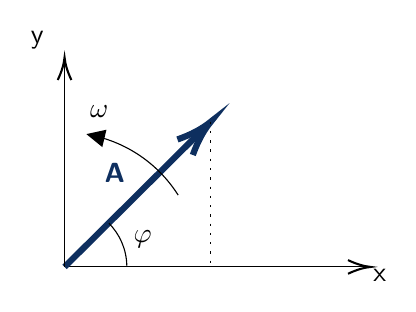
\begin{tikzpicture}[x=0.75pt,y=0.75pt,yscale=-1,xscale=1]
%uncomment if require: \path (0,15225); %set diagram left start at 0, and has height of 15225

%Straight Lines [id:da5927370156317948] 
\draw    (220,933) -- (365.5,933) ;
\draw [shift={(367.5,933)}, rotate = 180] [color={rgb, 255:red, 0; green, 0; blue, 0 }  ][line width=0.75]    (10.93,-3.29) .. controls (6.95,-1.4) and (3.31,-0.3) .. (0,0) .. controls (3.31,0.3) and (6.95,1.4) .. (10.93,3.29)   ;
%Straight Lines [id:da34962116656860287] 
\draw [color={BlueDefault}  ,draw opacity=1 ][line width=2.25]    (220,933) -- (287.66,865.82) ;
\draw [shift={(290.5,863)}, rotate = 135.2] [color={BlueDefault}   ,draw opacity=1 ][line width=2.25]    (17.49,-5.26) .. controls (11.12,-2.23) and (5.29,-0.48) .. (0,0) .. controls (5.29,0.48) and (11.12,2.23) .. (17.49,5.26)   ;
%Shape: Arc [id:dp021810946519202234] 
\draw  [draw opacity=0] (241.38,911.96) .. controls (246.57,917.22) and (249.82,924.39) .. (249.99,932.32) -- (220,933) -- cycle ; \draw   (241.38,911.96) .. controls (246.57,917.22) and (249.82,924.39) .. (249.99,932.32) ;  
%Shape: Arc [id:dp8513799267562083] 
\draw  [draw opacity=0] (238,870.79) .. controls (253.36,875.22) and (266.37,885.19) .. (274.73,898.39) -- (220,933) -- cycle ; \draw   (238,870.79) .. controls (253.36,875.22) and (266.37,885.19) .. (274.73,898.39) ;  
%Straight Lines [id:da8048233056164524] 
\draw    (238,870.79) -- (233.42,869.69) ;
\draw [shift={(230.5,869)}, rotate = 13.39] [fill={rgb, 255:red, 0; green, 0; blue, 0 }  ][line width=0.08]  [draw opacity=0] (8.93,-4.29) -- (0,0) -- (8.93,4.29) -- cycle    ;
%Straight Lines [id:da8962545520745455] 
\draw    (220,933) -- (220,834) ;
\draw [shift={(220,832)}, rotate = 90] [color={rgb, 255:red, 0; green, 0; blue, 0 }  ][line width=0.75]    (10.93,-3.29) .. controls (6.95,-1.4) and (3.31,-0.3) .. (0,0) .. controls (3.31,0.3) and (6.95,1.4) .. (10.93,3.29)   ;
%Straight Lines [id:da4834893344127229] 
\draw  [dash pattern={on 0.84pt off 2.51pt}]  (290.5,863) -- (290.5,933) ;

% Text Node
\draw (367.5,933) node [anchor=north west][inner sep=0.75pt]   [align=left] {x};
% Text Node
\draw (231,854) node [anchor=north west][inner sep=0.75pt]    {$\omega $};
% Text Node
\draw (252,914) node [anchor=north west][inner sep=0.75pt]    {$\varphi $};
% Text Node
\draw (238,882) node [anchor=north west][inner sep=0.75pt]   [align=left] {\textbf{\textcolor{BlueDefault}{A}}};
% Text Node
\draw (202.5,818) node [anchor=north west][inner sep=0.75pt]   [align=left] {y};


\end{tikzpicture}}
        \end{minipage}
        \hspace{1mm}
        \begin{minipage}{0.4\linewidth}
        \resizebox{1\linewidth}{!}{


\tikzset{every picture/.style={line width=0.75pt}} %set default line width to 0.75pt        

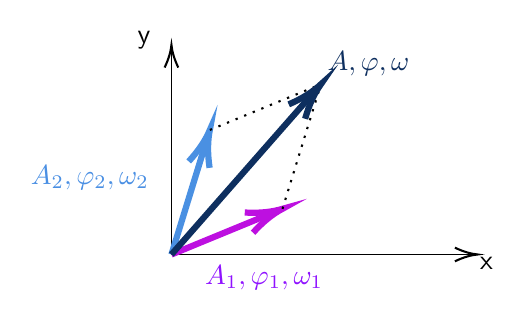
\begin{tikzpicture}[x=0.75pt,y=0.75pt,yscale=-1,xscale=1]
%uncomment if require: \path (0,15225); %set diagram left start at 0, and has height of 15225

%Straight Lines [id:da5927370156317948] 
\draw    (146,906) -- (291.5,906) ;
\draw [shift={(293.5,906)}, rotate = 180] [color={rgb, 255:red, 0; green, 0; blue, 0 }  ][line width=0.75]    (10.93,-3.29) .. controls (6.95,-1.4) and (3.31,-0.3) .. (0,0) .. controls (3.31,0.3) and (6.95,1.4) .. (10.93,3.29)   ;
%Straight Lines [id:da34962116656860287] 
\draw [color={rgb, 255:red, 189; green, 16; blue, 224 }  ,draw opacity=1 ][line width=2.25]    (146,906) -- (195.8,885.52) ;
\draw [shift={(199.5,884)}, rotate = 157.65] [color={rgb, 255:red, 189; green, 16; blue, 224 }  ,draw opacity=1 ][line width=2.25]    (17.49,-5.26) .. controls (11.12,-2.23) and (5.29,-0.48) .. (0,0) .. controls (5.29,0.48) and (11.12,2.23) .. (17.49,5.26)   ;
%Shape: Arc [id:dp021810946519202234] 
%\draw  [draw opacity=0] (192.38,889.39) .. controls (194.24,894.58) and (195.25,900.17) .. (195.25,906) -- (146,906) -- cycle ; \draw  [color={rgb, 255:red, 144; green, 19; blue, 254 }  ,draw opacity=1 ] (192.38,889.39) .. controls (194.24,894.58) and (195.25,900.17) .. (195.25,906) ;  
%Straight Lines [id:da8962545520745455] 
\draw    (146,906) -- (146,807) ;
\draw [shift={(146,805)}, rotate = 90] [color={rgb, 255:red, 0; green, 0; blue, 0 }  ][line width=0.75]    (10.93,-3.29) .. controls (6.95,-1.4) and (3.31,-0.3) .. (0,0) .. controls (3.31,0.3) and (6.95,1.4) .. (10.93,3.29)   ;
%Straight Lines [id:da9101145846792975] 
\draw [color={rgb, 255:red, 74; green, 144; blue, 226 }  ,draw opacity=1 ][line width=2.25]    (146,906) -- (163.32,849.82) ;
\draw [shift={(164.5,846)}, rotate = 107.14] [color={rgb, 255:red, 74; green, 144; blue, 226 }  ,draw opacity=1 ][line width=2.25]    (17.49,-5.26) .. controls (11.12,-2.23) and (5.29,-0.48) .. (0,0) .. controls (5.29,0.48) and (11.12,2.23) .. (17.49,5.26)   ;
%Straight Lines [id:da7014505903865442] 
\draw [color={rgb, 255:red, 0; green, 0; blue, 0 }  ,draw opacity=1 ][line width=0.75]  [dash pattern={on 0.84pt off 2.51pt}]  (199.5,884) -- (218,824) ;
%Straight Lines [id:da16436515246039618] 
\draw [color={rgb, 255:red, 0; green, 0; blue, 0 }  ,draw opacity=1 ][line width=0.75]  [dash pattern={on 0.84pt off 2.51pt}]  (164.5,846) -- (218,824) ;
%Straight Lines [id:da04823563439608747] 
\draw [color={BlueDefault}  ,draw opacity=1 ][line width=2.25]    (146,906) -- (215.36,827.01) ;
\draw [shift={(218,824)}, rotate = 131.28] [color={BlueDefault}  ,draw opacity=1 ][line width=2.25]    (17.49,-5.26) .. controls (11.12,-2.23) and (5.29,-0.48) .. (0,0) .. controls (5.29,0.48) and (11.12,2.23) .. (17.49,5.26)   ;
%Shape: Arc [id:dp07991088679681413] 
%\draw  [draw opacity=0] (174,875.54) .. controls (182.22,883.1) and (187.38,893.95) .. (187.38,906) -- (146,906) -- cycle ; \draw  [color={BlueDefault}  ,draw opacity=1 ] (174,875.54) .. controls (182.22,883.1) and (187.38,893.95) .. (187.38,906) ;  
%Shape: Arc [id:dp23775076053933653] 
%\draw  [draw opacity=0] (155.25,876) .. controls (167.91,880.28) and (177.15,891.99) .. (177.78,905.94) -- (144.62,907.45) -- cycle ; \draw  [color={rgb, 255:red, 74; green, 144; blue, 226 }  ,draw opacity=1 ] (155.25,876) .. controls (167.91,880.28) and (177.15,891.99) .. (177.78,905.94) ;  

% Text Node
\draw (293.5,906) node [anchor=north west][inner sep=0.75pt]   [align=left] {x};
% Text Node
\draw (129,863) node [anchor=north west][inner sep=0.75pt]   [align=left] {};
% Text Node
\draw (128.5,797) node [anchor=north west][inner sep=0.75pt]   [align=left] {y};
% Text Node
\draw (77,862) node [anchor=north west][inner sep=0.75pt]    {$\textcolor[rgb]{0.29,0.56,0.89}{A_{2} ,\varphi _{2} ,\omega _{2} \ }$};
% Text Node
\draw (161,910) node [anchor=north west][inner sep=0.75pt]    {$\textcolor[rgb]{0.56,0.07,1}{A_{1} ,\varphi _{1} ,\omega _{1}}$};
% Text Node
\draw (220,807) node [anchor=north west][inner sep=0.75pt]    {$\textcolor{BlueDefault}{A,\varphi ,\omega }$};


\end{tikzpicture}}
        \end{minipage}
    \end{center}
    Ta có thể biểu diễn phương trình dao động như một vector với giản đồ Fresnel.
\end{frame}

\section{Dao động liên kết}
\subsection{Hai khối lượng - ba lò xo}
\begin{frame}{2 khối lượng - 3 lò xo}
    Hệ dao động liên kết cơ bản đầu tiên chúng ta tìm hiểu là hệ 2 khối lượng 3 lò xo. Bỏ qua độ dài tự nhiên của lò xo.
    \vspace{2mm}
    \begin{center}
        \scalebox{1}{


% Pattern Info
 
\tikzset{
pattern size/.store in=\mcSize, 
pattern size = 5pt,
pattern thickness/.store in=\mcThickness, 
pattern thickness = 0.3pt,
pattern radius/.store in=\mcRadius, 
pattern radius = 1pt}
\makeatletter
\pgfutil@ifundefined{pgf@pattern@name@_mysjemblw}{
\pgfdeclarepatternformonly[\mcThickness,\mcSize]{_mysjemblw}
{\pgfqpoint{0pt}{0pt}}
{\pgfpoint{\mcSize+\mcThickness}{\mcSize+\mcThickness}}
{\pgfpoint{\mcSize}{\mcSize}}
{
\pgfsetcolor{\tikz@pattern@color}
\pgfsetlinewidth{\mcThickness}
\pgfpathmoveto{\pgfqpoint{0pt}{0pt}}
\pgfpathlineto{\pgfpoint{\mcSize+\mcThickness}{\mcSize+\mcThickness}}
\pgfusepath{stroke}
}}
\makeatother

% Pattern Info
 
\tikzset{
pattern size/.store in=\mcSize, 
pattern size = 5pt,
pattern thickness/.store in=\mcThickness, 
pattern thickness = 0.3pt,
pattern radius/.store in=\mcRadius, 
pattern radius = 1pt}
\makeatletter
\pgfutil@ifundefined{pgf@pattern@name@_mggpvl8gd}{
\pgfdeclarepatternformonly[\mcThickness,\mcSize]{_mggpvl8gd}
{\pgfqpoint{0pt}{0pt}}
{\pgfpoint{\mcSize+\mcThickness}{\mcSize+\mcThickness}}
{\pgfpoint{\mcSize}{\mcSize}}
{
\pgfsetcolor{\tikz@pattern@color}
\pgfsetlinewidth{\mcThickness}
\pgfpathmoveto{\pgfqpoint{0pt}{0pt}}
\pgfpathlineto{\pgfpoint{\mcSize+\mcThickness}{\mcSize+\mcThickness}}
\pgfusepath{stroke}
}}
\makeatother
\tikzset{every picture/.style={line width=0.75pt}} %set default line width to 0.75pt        

\begin{tikzpicture}[x=0.75pt,y=0.75pt,yscale=-1,xscale=1]
%uncomment if require: \path (0,15225); %set diagram left start at 0, and has height of 15225

%Straight Lines [id:da3223058949903339] 
\draw    (446.5,1088.22) -- (86,1088.22) ;
%Shape: Rectangle [id:dp7648671038082127] 
\draw  [draw opacity=0][pattern=_mysjemblw,pattern size=6pt,pattern thickness=0.75pt,pattern radius=0pt, pattern color={rgb, 255:red, 0; green, 0; blue, 0}] (86,1047) -- (60.5,1047) -- (60.5,1088.22) -- (86,1088.22) -- cycle ;
%Shape: Resistor [id:dp6479321963022213] 
\draw   (86,1067.61) -- (102.65,1067.61) -- (106.35,1058.73) -- (113.75,1076.48) -- (121.15,1058.73) -- (128.55,1076.48) -- (135.95,1058.73) -- (143.35,1076.48) -- (150.75,1058.73) -- (158.15,1076.48) -- (161.85,1067.61) -- (178.5,1067.61) ;
%Shape: Square [id:dp15263822722006148] 
\draw   (178.5,1047) -- (219.72,1047) -- (219.72,1088.22) -- (178.5,1088.22) -- cycle ;
%Shape: Resistor [id:dp3406372469944945] 
\draw   (220,1067.61) -- (236.65,1067.61) -- (240.35,1058.73) -- (247.75,1076.48) -- (255.15,1058.73) -- (262.55,1076.48) -- (269.95,1058.73) -- (277.35,1076.48) -- (284.75,1058.73) -- (292.15,1076.48) -- (295.85,1067.61) -- (312.5,1067.61) ;
%Shape: Square [id:dp8671738733511334] 
\draw   (312.5,1047) -- (353.72,1047) -- (353.72,1088.22) -- (312.5,1088.22) -- cycle ;
%Shape: Resistor [id:dp4210341004898319] 
\draw   (354,1067.61) -- (370.65,1067.61) -- (374.35,1058.73) -- (381.75,1076.48) -- (389.15,1058.73) -- (396.55,1076.48) -- (403.95,1058.73) -- (411.35,1076.48) -- (418.75,1058.73) -- (426.15,1076.48) -- (429.85,1067.61) -- (446.5,1067.61) ;
%Straight Lines [id:da6091760378667466] 
\draw    (86,1047) -- (86,1088.22) ;
%Straight Lines [id:da1853906688587692] 
\draw    (446.5,1047) -- (446.5,1088.22) ;
%Shape: Rectangle [id:dp9695945528994532] 
\draw  [draw opacity=0][pattern=_mggpvl8gd,pattern size=6pt,pattern thickness=0.75pt,pattern radius=0pt, pattern color={rgb, 255:red, 0; green, 0; blue, 0}] (472,1047) -- (446.5,1047) -- (446.5,1088.22) -- (472,1088.22) -- cycle ;
%Straight Lines [id:da6417307585486507] 
\draw    (201,1118) -- (238.5,1118) ;
\draw [shift={(240.5,1118)}, rotate = 180] [color={rgb, 255:red, 0; green, 0; blue, 0 }  ][line width=0.75]    (10.93,-3.29) .. controls (6.95,-1.4) and (3.31,-0.3) .. (0,0) .. controls (3.31,0.3) and (6.95,1.4) .. (10.93,3.29)   ;
\draw [shift={(201,1118)}, rotate = 180] [color={rgb, 255:red, 0; green, 0; blue, 0 }  ][line width=0.75]    (0,5.59) -- (0,-5.59)   ;
%Straight Lines [id:da15068921372551158] 
\draw    (332,1118) -- (369.5,1118) ;
\draw [shift={(371.5,1118)}, rotate = 180] [color={rgb, 255:red, 0; green, 0; blue, 0 }  ][line width=0.75]    (10.93,-3.29) .. controls (6.95,-1.4) and (3.31,-0.3) .. (0,0) .. controls (3.31,0.3) and (6.95,1.4) .. (10.93,3.29)   ;
\draw [shift={(332,1118)}, rotate = 180] [color={rgb, 255:red, 0; green, 0; blue, 0 }  ][line width=0.75]    (0,5.59) -- (0,-5.59)   ;

% Text Node
\draw (127,1036.22) node [anchor=north west][inner sep=0.75pt]   [align=left] {$\displaystyle k_{1}$};
% Text Node
\draw (199.11,1067.61) node   [align=left] {$\displaystyle m_{1}$};
% Text Node
\draw (333.11,1067.61) node   [align=left] {$\displaystyle m_{2}$};
% Text Node
\draw (201,1129) node [anchor=north west][inner sep=0.75pt]    {$x_{1}$};
% Text Node
\draw (332,1129) node [anchor=north west][inner sep=0.75pt]    {$x_{2}$};
% Text Node
\draw (258,1036.2) node [anchor=north west][inner sep=0.75pt]   [align=left] {$\displaystyle k_{2}$};
% Text Node
\draw (390,1036.2) node [anchor=north west][inner sep=0.75pt]   [align=left] {$\displaystyle k_{3}$};


\end{tikzpicture}}
    \end{center}
    Tổng hợp lực tác dụng lên $m_1$ và $m_2$ là
    \begin{equation}
    \left\{
    \begin{array}{ccc}
    m_1 x_1'' &=& - k_1 x_1 + k_2 (x_2 - x_1) \\
    m_2 x_2'' &=& - k_3 x_2 + k_2 (x_1 - x_2).
    \end{array}
    \right.
    \label{3.1_1}
    \end{equation}
\end{frame}

\begin{frame}{2 khối lượng - 3 lò xo}
    Ta xét trường hợp đơn giản $k_1 = k_3$, $m_1 = m_2 = m$. 

    Cách 1: Thay trường hợp trên vào, ta thu được hệ
    \begin{equation}
    \left\{
    \begin{array}{ccc}
    m_1 x_1'' &=& - k_1 x_1 + k_2 (x_2 - x_1) \\
    m_2 x_2'' &=& - k_1 x_2 + k_2 (x_1 - x_2).
    \end{array}
    \right.
    \label{3.1_2}
    \end{equation}
    Để giải hệ phương trình trên, ta lấy lần lượt tính $(x_1'' - x_2'')$ và $(x_1''+x_2'')$.
    \begin{equation}
    \left\{
        \begin{array}{ccc}
        m(x_1''+x_2'') &=& -k_1(x_1+x_2) \\
        m(x_1''-x_2'') &=& -(k_1+k_2)(x_1 - x_2).
        \end{array}
    \right.
    \end{equation}
    
\end{frame}

\subsection{Toạ độ suy rộng}
\begin{frame}{Không gian \(\mathcal{X}\)}
    \begin{center}
        \begin{minipage}{0.4\linewidth}
            \begin{center}
                \resizebox{1\linewidth}{!}{


\tikzset{every picture/.style={line width=0.75pt}} %set default line width to 0.75pt        

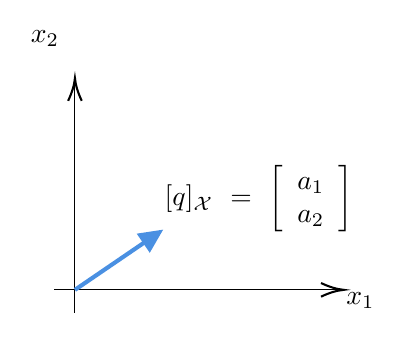
\begin{tikzpicture}[x=0.75pt,y=0.75pt,yscale=-1,xscale=1]
%uncomment if require: \path (0,15225); %set diagram left start at 0, and has height of 15225

%Straight Lines [id:da30187225832710496] 
\draw    (283,3620) -- (420.5,3620) ;
\draw [shift={(422.5,3620)}, rotate = 180] [color={rgb, 255:red, 0; green, 0; blue, 0 }  ][line width=0.75]    (10.93,-3.29) .. controls (6.95,-1.4) and (3.31,-0.3) .. (0,0) .. controls (3.31,0.3) and (6.95,1.4) .. (10.93,3.29)   ;
%Straight Lines [id:da7150609245229815] 
\draw    (293,3631) -- (293,3620) -- (293,3520) ;
\draw [shift={(293,3518)}, rotate = 90] [color={rgb, 255:red, 0; green, 0; blue, 0 }  ][line width=0.75]    (10.93,-3.29) .. controls (6.95,-1.4) and (3.31,-0.3) .. (0,0) .. controls (3.31,0.3) and (6.95,1.4) .. (10.93,3.29)   ;
%Straight Lines [id:da12230210739845826] 
\draw [color={rgb, 255:red, 74; green, 144; blue, 226 }  ,draw opacity=1 ][line width=1.5]    (293,3620) -- (332.2,3593.25) ;
\draw [shift={(335.5,3591)}, rotate = 145.69] [fill={rgb, 255:red, 74; green, 144; blue, 226 }  ,fill opacity=1 ][line width=0.08]  [draw opacity=0] (11.61,-5.58) -- (0,0) -- (11.61,5.58) -- cycle    ;

% Text Node
\draw (422.5,3620) node [anchor=north west][inner sep=0.75pt]    {$x_{1}$};
% Text Node
\draw (270.5,3494) node [anchor=north west][inner sep=0.75pt]    {$x_{2}$};
% Text Node
\draw (335,3559) node [anchor=north west][inner sep=0.75pt]    {$[ q]_{\mathcal{X}} \ =\ 
\left[
\begin{array}{c}
a_1 \\ a_2
\end{array} \right] $};


\end{tikzpicture}}
            \end{center}
        \end{minipage}
        \hspace{1mm}
        \begin{minipage}{0.4\linewidth}
            Gọi \(q\) là một vector trong không gian \(\mathcal{X}\). \(q\) là một tổ hợp tuyến tính 
            \begin{equation}
                q = \sum_{i=1}^{2} a_i x_i.
                \label{eq:3.2}
            \end{equation}
        \end{minipage}
    \end{center}
\end{frame}

\subsection{Ma trận ánh xạ định luật II Newton}
\input{Content/Dao động liên kết/3.3}

\subsection{Ý tưởng chính}
\begin{frame}{Ý tưởng chính}
    Để nó có thể xuất hiện phương trình giống với phương trình dao động, ta mong muốn ánh xạ $\mathbf{[M]^{-1}}\mathbf{[K]}$ sẽ "bảo toàn hệ số".
    \begin{center}
        \resizebox{0.8\linewidth}{!}{


\tikzset{every picture/.style={line width=0.75pt}} %set default line width to 0.75pt        

\begin{tikzpicture}[x=0.75pt,y=0.75pt,yscale=-1,xscale=1]
%uncomment if require: \path (0,15225); %set diagram left start at 0, and has height of 15225

%Straight Lines [id:da46971419391016966] 
\draw    (155,5164) -- (155,5061) ;
\draw [shift={(155,5059)}, rotate = 90] [color={rgb, 255:red, 0; green, 0; blue, 0 }  ][line width=0.75]    (10.93,-3.29) .. controls (6.95,-1.4) and (3.31,-0.3) .. (0,0) .. controls (3.31,0.3) and (6.95,1.4) .. (10.93,3.29)   ;
%Straight Lines [id:da03406383173301375] 
\draw    (155,5164) -- (279.5,5164) ;
\draw [shift={(281.5,5164)}, rotate = 180] [color={rgb, 255:red, 0; green, 0; blue, 0 }  ][line width=0.75]    (10.93,-3.29) .. controls (6.95,-1.4) and (3.31,-0.3) .. (0,0) .. controls (3.31,0.3) and (6.95,1.4) .. (10.93,3.29)   ;
%Straight Lines [id:da495111073609535] 
\draw    (155,5164) -- (220.57,5146.52) ;
\draw [shift={(222.5,5146)}, rotate = 165.07] [color={rgb, 255:red, 0; green, 0; blue, 0 }  ][line width=0.75]    (10.93,-3.29) .. controls (6.95,-1.4) and (3.31,-0.3) .. (0,0) .. controls (3.31,0.3) and (6.95,1.4) .. (10.93,3.29)   ;
%Curve Lines [id:da4396149957962707] 
\draw    (300,5039.5) .. controls (325.71,5023.01) and (371.17,5021.57) .. (395.32,5037.93) ;
\draw [shift={(397.5,5039.5)}, rotate = 217.45] [fill={rgb, 255:red, 0; green, 0; blue, 0 }  ][line width=0.08]  [draw opacity=0] (8.93,-4.29) -- (0,0) -- (8.93,4.29) -- cycle    ;
%Straight Lines [id:da12429100250589431] 
\draw    (384,5165) -- (384,5062) ;
\draw [shift={(384,5060)}, rotate = 90] [color={rgb, 255:red, 0; green, 0; blue, 0 }  ][line width=0.75]    (10.93,-3.29) .. controls (6.95,-1.4) and (3.31,-0.3) .. (0,0) .. controls (3.31,0.3) and (6.95,1.4) .. (10.93,3.29)   ;
%Straight Lines [id:da011617708076129607] 
\draw    (384,5165) -- (508.5,5165) ;
\draw [shift={(510.5,5165)}, rotate = 180] [color={rgb, 255:red, 0; green, 0; blue, 0 }  ][line width=0.75]    (10.93,-3.29) .. controls (6.95,-1.4) and (3.31,-0.3) .. (0,0) .. controls (3.31,0.3) and (6.95,1.4) .. (10.93,3.29)   ;
%Straight Lines [id:da8611613220381794] 
\draw    (384,5165) -- (449.57,5147.52) ;
\draw [shift={(451.5,5147)}, rotate = 165.07] [color={rgb, 255:red, 0; green, 0; blue, 0 }  ][line width=0.75]    (10.93,-3.29) .. controls (6.95,-1.4) and (3.31,-0.3) .. (0,0) .. controls (3.31,0.3) and (6.95,1.4) .. (10.93,3.29)   ;

% Text Node
\draw (219,5032) node [anchor=north west][inner sep=0.75pt]  [font=\Large]  {$\mathcal{X}$};
% Text Node
\draw (212,5104) node [anchor=north west][inner sep=0.75pt]    {$[ q]_{\mathcal{X}} \ =
\left[
\begin{array}{c}
a _{1}\\
a _{2}
\end{array} 
\right]  $};
% Text Node
\draw (310,5001.5) node [anchor=north west][inner sep=0.75pt]    {$\mathbf{[M]^{-1}}\mathbf{[K]}$};
% Text Node
\draw (441,5105) node [anchor=north west][inner sep=0.75pt]    {$[ q'']_{\mathcal{X} ''} \ =\alpha \left[
\begin{array}{c}
a _{1}\\
a _{2}
\end{array} 
\right]  $};
% Text Node
\draw (459,5032) node [anchor=north west][inner sep=0.75pt]  [font=\Large]  {$\mathcal{X}^{''}$};


\end{tikzpicture}
}
    \end{center}
\end{frame}
\begin{frame}{Ý tưởng chính}
    Bây giờ, ta sẽ giả sử những điều sau
    \begin{enumerate}[\textbullet]
        \item \(x_1 = A e^{\lambda t}  ; \ x_2 = B e^{\lambda t} \Rightarrow [q]_{\mathcal{X}} = 
            \left[
            \begin{array}{c}
            A  \\
            B 
            \end{array} \right] \) \cite{morin2008introduction} \cite{taylor2005classic}
        \item Thoả điều kiện "bảo toàn hệ số".
    \end{enumerate}
    Nếu thoả điều kiện hai, thì ta có thể viết
    \begin{equation}
        [q'']_{\mathcal{X}''} = \lambda^2             
        \left[
            \begin{array}{c}
            A  \\
            B 
            \end{array} 
        \right].
        \label{eq:3.4_1}
    \end{equation}
    Đưa vào phương trình (\ref{eq:3.3_3}), ta có
    \begin{equation}
        \Big(\mathbf{[K]} - \lambda^2 \mathbf{[M]}\Big) 
        \left[
            \begin{array}{c}
            A  \\
            B 
            \end{array} 
        \right] = 0.
        \label{eq:3.4_2}
    \end{equation}
\end{frame}

\begin{frame}{Chéo hoá ma trận}
    Ta tìm hiểu về khái niệm Eigenvalue và Eigenvector. \cite{gilbert2009introduction}
    \vspace{2mm}

    Cho phép toán sau, với \(\mathbf{[A]}\) là ma trận ánh xạ tuyến tính; \(\mathbf{v}\) là vector
    \begin{equation}
        \mathbf{[A]} \mathbf{v} = \lambda \mathbf{v} \ \ \text{Hay} \ \ \Big( \mathbf{[A]} - \lambda \mathbf{[E]} \Big) \mathbf{v} = 0
        \label{eq:3.4_3}
    \end{equation}
    Eigenvector, là những vector \(\mathbf{v}\) thoả phương trình trên; Eigenvalue, là những giá trị \(\lambda\) tương ứng với vector \(\mathbf{v}\) là Eigenvector.
    \vspace{2mm}

    \textbf{Bước 1:} Tìm giá trị \(\lambda\) thoả (tính chất nghiệm không tầm thường)
    \begin{equation}
        \det \Big( \mathbf{[A]} - \lambda \mathbf{[E]} \Big) = 0.
        \label{eq:3.4_4}
    \end{equation}
\end{frame}
\begin{frame}{Chéo hoá ma trận}
    \textbf{Bước 2:} Thay các giá trị \(\lambda\) vào phương trình (???) để tìm eigenvector \(\mathbf{v}\).
    \vspace{2mm}

    \textbf{Bước 3:} Ta thu được \(\lambda_1, \lambda_2\) và các vector \(\mathbf{v_1}, \mathbf{v_2}\). Ta sẽ viết được
    \begin{equation}
        \mathbf{[A]} = \left[\mathbf{v_1} \ \mathbf{v_2}\right] 
        \left[
        \begin{array}{cc}
        \lambda_1 & 0 \\
        0 & \lambda_2 
        \end{array}
        \right] \left[\mathbf{v_1} \ \mathbf{v_2}\right]^{-1}
        \label{3.4_5}
    \end{equation}
    \begin{center}
        \begin{minipage}{0.45\linewidth}
            \textbf{Ví dụ:} Chéo hoá ma trận \(\mathbf{[B]}\).
            \begin{equation*}
                \mathbf{[B]} = 
                \left[
                \begin{array}{cc}
                    3 & -3 \\
                    2 & -4
                \end{array}
                \right]
            \end{equation*}
            \pause
            \textbf{Giải}

            B1: giải \(\det \Big(\mathbf{[B]} - \lambda \mathbf{[E]} \Big)=0\), ta có \(\lambda = 2,-3\).
        \end{minipage}
        \hspace{5mm}
        \begin{minipage}{0.45\linewidth}
            B2: Với \(\lambda = 2\), ta giải hệ \(\left[
            \begin{array}{cc}
                3 - 2 & -3 \\
                2 & -4 -2
            \end{array}\right] \left[
            \begin{array}{c}
            A \\
            B
            \end{array}\right] = 0\)
            \vspace{2mm}

            \(\rightarrow \mathbf{v_1} = \left[
            \begin{array}{c}
            A \\
            B
            \end{array}\right] = \left[
            \begin{array}{c}
            3 \\
            1
            \end{array}\right] \)
        \end{minipage}
    \end{center}
\end{frame}
\begin{frame}{Chéo hoá ma trận}
    \textbf{Bước 2:} Thay các giá trị \(\lambda\) vào phương trình (???) để tìm eigenvector \(\mathbf{v}\).
    \vspace{2mm}

    \textbf{Bước 3:} Ta thu được \(\lambda_1, \lambda_2\) và các vector \(\mathbf{v_1}, \mathbf{v_2}\). Ta sẽ viết được
    \begin{equation}
        \mathbf{[A]} = \left[\mathbf{v_1} \ \mathbf{v_2}\right] 
        \left[
        \begin{array}{cc}
        \lambda_1 & 0 \\
        0 & \lambda_2 
        \end{array}
        \right] \left[\mathbf{v_1} \ \mathbf{v_2}\right]^{-1}
        \label{eq:3.4_6}
    \end{equation}
    \begin{center}
        \begin{minipage}{0.45\linewidth}
            \textbf{Ví dụ:} Chéo hoá ma trận \(\mathbf{[B]}\).
            \begin{equation*}
                \mathbf{[B]} = 
                \left[
                \begin{array}{cc}
                    3 & -3 \\
                    2 & -4
                \end{array}
                \right]
            \end{equation*}
            \textbf{Giải}

            B1: giải \(\det \Big(\mathbf{[B]} - \lambda \mathbf{[E]} \Big)=0\), ta có \(\lambda = 2,-3\).
        \end{minipage}
        \hspace{5mm}
        \begin{minipage}{0.45\linewidth}
            B2: Tương tự, với \(\lambda = -3 \ \text{thì}\) 
            \vspace{2mm}
            
            \( \mathbf{v_2} = \left[
            \begin{array}{c}
            A \\
            B
            \end{array}\right] = \left[
            \begin{array}{c}
            1 \\
            2
            \end{array}\right]  \)

            B3: \[\mathbf{[B]} = \left[
                \begin{array}{cc}
                    3 & 1 \\
                    1 & 2
                \end{array}
                \right]                 
                \left[
                \begin{array}{cc}
                    2 & 0 \\
                    0 & -3
                \end{array}
                \right]                
                \left[
                \begin{array}{cc}
                    3 & 1 \\
                    1 & 2
                \end{array}
                \right]^{-1}
                \]
        \end{minipage}
    \end{center}
\end{frame}
\begin{frame}{Ý tưởng chính}

    Chúng ta sẽ tìm \(\lambda\) để thoả mãn phương trình (\ref{eq:3.4_2}), ta có tính chất nghiệm không tầm thường
    \begin{equation}
        \det{\Big( \mathbf{[K]} - \lambda^2 \mathbf{[M]}\Big)} = 0.
        \label{eq:3.4_7}
    \end{equation}
    Sau giải ra được \(\lambda\), ta thế chúng ngược lại để tìm vector \(q\) tương ứng. Những vector \(q\) được gọi là \textit{toạ độ trực giao}. Hoặc còn gọi là các \textbf{mode dao động}.
\end{frame}

\begin{frame}{Nghiệm tổng quát}
    Giả sử ta tìm được n vector \(q\), ứng với mỗi vector \(q_i\) có \(k_i\) trị riêng \(\lambda\) (eigenvalue). \(\lambda_{ij}\) là trị riêng thứ \(j\) ứng với vector \(q_i\).
    \begin{equation}
    q_{tq} = 
    \left[\begin{array}{c}
    x_1 \\ x_2
    \end{array}\right] \displaystyle = q_1 \sum_{i=0}^{k_1} A_{1i} e^{\lambda_{1i} t} + ... +  q_n \sum_{i=1}^{k_n} A_{ni} e^{\lambda_{ni} t}
    \label{eq:3.4_8}
    \end{equation}
\end{frame}

\section{Bài tập}
\begin{frame}{Bài 1}
Giải lại hệ sau bằng phương pháp chéo hoá. Với \(m_1=m_2=m\), \(k_1=k_3=2k_2\).
\begin{center}
    \resizebox{1\linewidth}{!}{


% Pattern Info
 
\tikzset{
pattern size/.store in=\mcSize, 
pattern size = 5pt,
pattern thickness/.store in=\mcThickness, 
pattern thickness = 0.3pt,
pattern radius/.store in=\mcRadius, 
pattern radius = 1pt}
\makeatletter
\pgfutil@ifundefined{pgf@pattern@name@_mysjemblw}{
\pgfdeclarepatternformonly[\mcThickness,\mcSize]{_mysjemblw}
{\pgfqpoint{0pt}{0pt}}
{\pgfpoint{\mcSize+\mcThickness}{\mcSize+\mcThickness}}
{\pgfpoint{\mcSize}{\mcSize}}
{
\pgfsetcolor{\tikz@pattern@color}
\pgfsetlinewidth{\mcThickness}
\pgfpathmoveto{\pgfqpoint{0pt}{0pt}}
\pgfpathlineto{\pgfpoint{\mcSize+\mcThickness}{\mcSize+\mcThickness}}
\pgfusepath{stroke}
}}
\makeatother

% Pattern Info
 
\tikzset{
pattern size/.store in=\mcSize, 
pattern size = 5pt,
pattern thickness/.store in=\mcThickness, 
pattern thickness = 0.3pt,
pattern radius/.store in=\mcRadius, 
pattern radius = 1pt}
\makeatletter
\pgfutil@ifundefined{pgf@pattern@name@_mggpvl8gd}{
\pgfdeclarepatternformonly[\mcThickness,\mcSize]{_mggpvl8gd}
{\pgfqpoint{0pt}{0pt}}
{\pgfpoint{\mcSize+\mcThickness}{\mcSize+\mcThickness}}
{\pgfpoint{\mcSize}{\mcSize}}
{
\pgfsetcolor{\tikz@pattern@color}
\pgfsetlinewidth{\mcThickness}
\pgfpathmoveto{\pgfqpoint{0pt}{0pt}}
\pgfpathlineto{\pgfpoint{\mcSize+\mcThickness}{\mcSize+\mcThickness}}
\pgfusepath{stroke}
}}
\makeatother
\tikzset{every picture/.style={line width=0.75pt}} %set default line width to 0.75pt        

\begin{tikzpicture}[x=0.75pt,y=0.75pt,yscale=-1,xscale=1]
%uncomment if require: \path (0,15225); %set diagram left start at 0, and has height of 15225

%Straight Lines [id:da3223058949903339] 
\draw    (446.5,1088.22) -- (86,1088.22) ;
%Shape: Rectangle [id:dp7648671038082127] 
\draw  [draw opacity=0][pattern=_mysjemblw,pattern size=6pt,pattern thickness=0.75pt,pattern radius=0pt, pattern color={rgb, 255:red, 0; green, 0; blue, 0}] (86,1047) -- (60.5,1047) -- (60.5,1088.22) -- (86,1088.22) -- cycle ;
%Shape: Resistor [id:dp6479321963022213] 
\draw   (86,1067.61) -- (102.65,1067.61) -- (106.35,1058.73) -- (113.75,1076.48) -- (121.15,1058.73) -- (128.55,1076.48) -- (135.95,1058.73) -- (143.35,1076.48) -- (150.75,1058.73) -- (158.15,1076.48) -- (161.85,1067.61) -- (178.5,1067.61) ;
%Shape: Square [id:dp15263822722006148] 
\draw   (178.5,1047) -- (219.72,1047) -- (219.72,1088.22) -- (178.5,1088.22) -- cycle ;
%Shape: Resistor [id:dp3406372469944945] 
\draw   (220,1067.61) -- (236.65,1067.61) -- (240.35,1058.73) -- (247.75,1076.48) -- (255.15,1058.73) -- (262.55,1076.48) -- (269.95,1058.73) -- (277.35,1076.48) -- (284.75,1058.73) -- (292.15,1076.48) -- (295.85,1067.61) -- (312.5,1067.61) ;
%Shape: Square [id:dp8671738733511334] 
\draw   (312.5,1047) -- (353.72,1047) -- (353.72,1088.22) -- (312.5,1088.22) -- cycle ;
%Shape: Resistor [id:dp4210341004898319] 
\draw   (354,1067.61) -- (370.65,1067.61) -- (374.35,1058.73) -- (381.75,1076.48) -- (389.15,1058.73) -- (396.55,1076.48) -- (403.95,1058.73) -- (411.35,1076.48) -- (418.75,1058.73) -- (426.15,1076.48) -- (429.85,1067.61) -- (446.5,1067.61) ;
%Straight Lines [id:da6091760378667466] 
\draw    (86,1047) -- (86,1088.22) ;
%Straight Lines [id:da1853906688587692] 
\draw    (446.5,1047) -- (446.5,1088.22) ;
%Shape: Rectangle [id:dp9695945528994532] 
\draw  [draw opacity=0][pattern=_mggpvl8gd,pattern size=6pt,pattern thickness=0.75pt,pattern radius=0pt, pattern color={rgb, 255:red, 0; green, 0; blue, 0}] (472,1047) -- (446.5,1047) -- (446.5,1088.22) -- (472,1088.22) -- cycle ;
%Straight Lines [id:da6417307585486507] 
\draw    (201,1118) -- (238.5,1118) ;
\draw [shift={(240.5,1118)}, rotate = 180] [color={rgb, 255:red, 0; green, 0; blue, 0 }  ][line width=0.75]    (10.93,-3.29) .. controls (6.95,-1.4) and (3.31,-0.3) .. (0,0) .. controls (3.31,0.3) and (6.95,1.4) .. (10.93,3.29)   ;
\draw [shift={(201,1118)}, rotate = 180] [color={rgb, 255:red, 0; green, 0; blue, 0 }  ][line width=0.75]    (0,5.59) -- (0,-5.59)   ;
%Straight Lines [id:da15068921372551158] 
\draw    (332,1118) -- (369.5,1118) ;
\draw [shift={(371.5,1118)}, rotate = 180] [color={rgb, 255:red, 0; green, 0; blue, 0 }  ][line width=0.75]    (10.93,-3.29) .. controls (6.95,-1.4) and (3.31,-0.3) .. (0,0) .. controls (3.31,0.3) and (6.95,1.4) .. (10.93,3.29)   ;
\draw [shift={(332,1118)}, rotate = 180] [color={rgb, 255:red, 0; green, 0; blue, 0 }  ][line width=0.75]    (0,5.59) -- (0,-5.59)   ;

% Text Node
\draw (127,1036.22) node [anchor=north west][inner sep=0.75pt]   [align=left] {$\displaystyle k_{1}$};
% Text Node
\draw (199.11,1067.61) node   [align=left] {$\displaystyle m_{1}$};
% Text Node
\draw (333.11,1067.61) node   [align=left] {$\displaystyle m_{2}$};
% Text Node
\draw (201,1129) node [anchor=north west][inner sep=0.75pt]    {$x_{1}$};
% Text Node
\draw (332,1129) node [anchor=north west][inner sep=0.75pt]    {$x_{2}$};
% Text Node
\draw (258,1036.2) node [anchor=north west][inner sep=0.75pt]   [align=left] {$\displaystyle k_{2}$};
% Text Node
\draw (390,1036.2) node [anchor=north west][inner sep=0.75pt]   [align=left] {$\displaystyle k_{3}$};


\end{tikzpicture}}
\end{center}
\end{frame}
\begin{frame}{Bài 1: Giải}
    Từ phương trình (\ref{eq:3.3_2}), ta có ma trận
    \begin{equation*}
    \left[
    \begin{array}{cc}
    -(k_1+k_2) & k_2 \\
    k_2 & -(k_1+ k_2)
    \end{array}
    \right] 
    \left[
    \begin{array}{c}
    x_1 \\
    x_2
    \end{array}
    \right] =  
    \left[
    \begin{array}{cc}
    m_1 & 0 \\
    0 & m_2 
    \end{array}
    \right] 
    \left[
    \begin{array}{c}
    x_1'' \\
    x_2''
    \end{array}
    \right]
    \end{equation*}
    Dựa vào giả thiết \(m_1=m_2=m\) và \(k_1 = k_3=2k_2\), ta tính định thức sau
    \begin{equation*}
        \det{\left(\left[
    \begin{array}{cc}
    -3 & 1 \\
    1 & -3
    \end{array}
    \right]  -  \frac{m}{k_2} \lambda^2 
    \left[
    \begin{array}{cc}
        1 & 0 \\
        0 & 1
    \end{array}
    \right]
    \right) 
    } = 0
    \end{equation*}
    Ta giải ra
    \begin{equation*}
    \begin{array}{clccc}
    &\displaystyle\frac{m}{k_2} \lambda^2 = -2 \ &\text{hoặc}&\displaystyle \ \frac{m}{k_2} \lambda^2=-4 \\
    \Rightarrow &\displaystyle \lambda= \pm i \sqrt{\frac{2k_2}{m}} \ &\text{hoặc}&\displaystyle \ \lambda = \pm i \sqrt{\frac{4k_2}{m}}
    \end{array}
    \end{equation*}
\end{frame}
\begin{frame}{Bài 1: Giải}
    Với \(\displaystyle \lambda= \pm i \sqrt{\frac{2k_2}{m}}\)
    \begin{equation*}
    \begin{array}{crc}
    &
    \left(\left[
    \begin{array}{cc}
    -3 & 1 \\
    1 & -3
    \end{array}
    \right]  +  2
    \left[
    \begin{array}{cc}
        1 & 0 \\
        0 & 1
    \end{array}
    \right]
    \right) \left[
    \begin{array}{c}
    x_1 \\ x_2
    \end{array}\right] &= 0 \\ \\
    \Rightarrow & 
    \left[
    \begin{array}{cc}
        -1 & 1 \\
        1 & -1
    \end{array}
    \right] \left[
    \begin{array}{c}
    x_1 \\
    x_2
    \end{array}\right] &=0 \\ \\
    \Rightarrow & x_1 &= x_2 
    \end{array}
    \end{equation*}
    Vậy vector riêng tương ứng là
    \begin{equation*}
        q_1 = \left[
        \begin{array}{c}
        1 \\
        1
        \end{array}
        \right]
    \end{equation*}
\end{frame}
\begin{frame}{Bài 1: Giải}
    Với \(\displaystyle \ \lambda = \pm i \sqrt{\frac{4k_2}{m}}\)
    \begin{equation*}
    \begin{array}{crc}
    &
    \left(\left[
    \begin{array}{cc}
    -3 & 1 \\
    1 & -3
    \end{array}
    \right]  +  4
    \left[
    \begin{array}{cc}
        1 & 0 \\
        0 & 1
    \end{array}
    \right]
    \right) \left[
    \begin{array}{c}
    x_1 \\ x_2
    \end{array}\right] &= 0 \\ \\
    \Rightarrow & 
    \left[
    \begin{array}{cc}
        1 & 1 \\
        1 & 1
    \end{array}
    \right] \left[
    \begin{array}{c}
    x_1 \\
    x_2
    \end{array}\right] &=0 \\ \\
    \Rightarrow & x_1 &= -x_2 
    \end{array}
    \end{equation*}
    Vậy vector riêng tương ứng là
    \begin{equation*}
        q_2 = \left[
        \begin{array}{c}
        1 \\
        -1
        \end{array}
        \right]
    \end{equation*}
\end{frame}
\begin{frame}{Bài 1: Giải}
    Nghiệm tổng quát
    \begin{equation*}
    \displaystyle
        q_{tq} = \left[
        \begin{array}{c}
        x_1 \\
        x_2
        \end{array}
        \right]
        = 
        \left[
        \begin{array}{c}
        1 \\ 1
        \end{array}
        \right] 
        \left( A_1 e^{i \sqrt{\frac{2k_2}{m}}t}  + A_2 e^{- i \sqrt{\frac{2k_2}{m}}t}\right) +  
        \left[
        \begin{array}{c}
        1 \\ -1
        \end{array}
        \right] \left( A_3 e^{ i \sqrt{\frac{4k_2}{m}}t} + A_4 e^{ - i \sqrt{\frac{4k_2}{m}}t}\right)
    \end{equation*}
    
\end{frame}
\begin{frame}{Bài 2}
Cho hệ con lắc, chúng được nối bởi một lò xo có độ cứng \(k\). Biết hệ dao động nhỏ và \(m_1=m_2=m\).
\begin{center}
    \resizebox{0.5\linewidth}{!}{


% Pattern Info
 
\tikzset{
pattern size/.store in=\mcSize, 
pattern size = 5pt,
pattern thickness/.store in=\mcThickness, 
pattern thickness = 0.3pt,
pattern radius/.store in=\mcRadius, 
pattern radius = 1pt}
\makeatletter
\pgfutil@ifundefined{pgf@pattern@name@_wij6wu0xe}{
\pgfdeclarepatternformonly[\mcThickness,\mcSize]{_wij6wu0xe}
{\pgfqpoint{0pt}{0pt}}
{\pgfpoint{\mcSize+\mcThickness}{\mcSize+\mcThickness}}
{\pgfpoint{\mcSize}{\mcSize}}
{
\pgfsetcolor{\tikz@pattern@color}
\pgfsetlinewidth{\mcThickness}
\pgfpathmoveto{\pgfqpoint{0pt}{0pt}}
\pgfpathlineto{\pgfpoint{\mcSize+\mcThickness}{\mcSize+\mcThickness}}
\pgfusepath{stroke}
}}
\makeatother
\tikzset{every picture/.style={line width=0.75pt}} %set default line width to 0.75pt        

\begin{tikzpicture}[x=0.75pt,y=0.75pt,yscale=-1,xscale=1]
%uncomment if require: \path (0,15225); %set diagram left start at 0, and has height of 15225

%Straight Lines [id:da4560813903220491] 
\draw    (192,6431) -- (308.5,6431) ;
%Straight Lines [id:da8433245400527029] 
\draw    (308.5,6431) -- (364.5,6431) ;
%Straight Lines [id:da387592998220613] 
\draw    (136,6431) -- (192,6431) ;
%Straight Lines [id:da9783671482224332] 
\draw    (192,6431) -- (210.5,6528) ;
%Straight Lines [id:da6978529644488559] 
\draw    (308.5,6431) -- (358.5,6528) ;
%Shape: Circle [id:dp3531244928501118] 
\draw  [draw opacity=0][fill={rgb, 255:red, 155; green, 155; blue, 155 }  ,fill opacity=1 ] (201,6528) .. controls (201,6522.75) and (205.25,6518.5) .. (210.5,6518.5) .. controls (215.75,6518.5) and (220,6522.75) .. (220,6528) .. controls (220,6533.25) and (215.75,6537.5) .. (210.5,6537.5) .. controls (205.25,6537.5) and (201,6533.25) .. (201,6528) -- cycle ;
%Shape: Circle [id:dp611050397633133] 
\draw  [draw opacity=0][fill={rgb, 255:red, 155; green, 155; blue, 155 }  ,fill opacity=1 ] (349,6528) .. controls (349,6522.75) and (353.25,6518.5) .. (358.5,6518.5) .. controls (363.75,6518.5) and (368,6522.75) .. (368,6528) .. controls (368,6533.25) and (363.75,6537.5) .. (358.5,6537.5) .. controls (353.25,6537.5) and (349,6533.25) .. (349,6528) -- cycle ;
%Straight Lines [id:da8476200129206126] 
\draw  [dash pattern={on 0.84pt off 2.51pt}]  (192,6431) -- (192,6490.5) ;
%Shape: Arc [id:dp8882181984382771] 
\draw  [draw opacity=0][fill={rgb, 255:red, 245; green, 166; blue, 35 }  ,fill opacity=1 ] (199.23,6469.08) .. controls (197.03,6469.49) and (194.77,6469.72) .. (192.47,6469.75) -- (192,6431) -- cycle ; \draw  [draw opacity=0] (199.23,6469.08) .. controls (197.03,6469.49) and (194.77,6469.72) .. (192.47,6469.75) ;  
%Straight Lines [id:da9639779470172831] 
\draw  [dash pattern={on 0.84pt off 2.51pt}]  (308.5,6431) -- (308.5,6490.5) ;
%Shape: Arc [id:dp059281678179842534] 
\draw  [draw opacity=0][fill={rgb, 255:red, 126; green, 211; blue, 33 }  ,fill opacity=1 ] (325.84,6465.67) .. controls (320.75,6468.21) and (315.03,6469.68) .. (308.97,6469.75) -- (308.5,6431) -- cycle ; \draw  [draw opacity=0] (325.84,6465.67) .. controls (320.75,6468.21) and (315.03,6469.68) .. (308.97,6469.75) ;  
%Shape: Resistor [id:dp6062120320253328] 
\draw   (220,6528) -- (243.22,6528) -- (248.38,6520.5) -- (258.7,6535.5) -- (269.02,6520.5) -- (279.34,6535.5) -- (289.66,6520.5) -- (299.98,6535.5) -- (310.3,6520.5) -- (320.62,6535.5) -- (325.78,6528) -- (349,6528) ;
%Shape: Rectangle [id:dp17811364608989888] 
\draw  [draw opacity=0][pattern=_wij6wu0xe,pattern size=6pt,pattern thickness=0.75pt,pattern radius=0pt, pattern color={rgb, 255:red, 0; green, 0; blue, 0}] (364.5,6422) -- (138.5,6422) -- (138.5,6431) -- (364.5,6431) -- cycle ;

% Text Node
\draw (168,6449) node [anchor=north west][inner sep=0.75pt]    {$\textcolor[rgb]{0.96,0.65,0.14}{\theta _{1}}$};
% Text Node
\draw (284,6449) node [anchor=north west][inner sep=0.75pt]    {$\textcolor[rgb]{0.49,0.83,0.13}{\theta _{2}}$};
% Text Node
\draw (208,6467) node [anchor=north west][inner sep=0.75pt]    {$L$};
% Text Node
\draw (343,6467) node [anchor=north west][inner sep=0.75pt]    {$L$};
% Text Node
\draw (198,6538) node [anchor=north west][inner sep=0.75pt]    {$m_{1}$};
% Text Node
\draw (347,6538) node [anchor=north west][inner sep=0.75pt]    {$m_{2}$};
% Text Node
\draw (271,6496.5) node [anchor=north west][inner sep=0.75pt]    {$k$};


\end{tikzpicture}}
\end{center}
\end{frame}
\begin{frame}{Bài 3}
Cho hệ như hình, thanh nối nằm ngang giữa các khối lượng coi như rất nhẹ. Các vật có khối lượng bằng nhau và bằng \(m\). Cho hệ dao động như hình, dao động đủ nhỏ để ta xem các thanh coi như các thanh không bị dịch chuyển theo phương thẳng đứng. 
\begin{center}
    \resizebox{0.8\linewidth}{!}{


% Pattern Info
 
\tikzset{
pattern size/.store in=\mcSize, 
pattern size = 5pt,
pattern thickness/.store in=\mcThickness, 
pattern thickness = 0.3pt,
pattern radius/.store in=\mcRadius, 
pattern radius = 1pt}
\makeatletter
\pgfutil@ifundefined{pgf@pattern@name@_62pu5u62w}{
\pgfdeclarepatternformonly[\mcThickness,\mcSize]{_62pu5u62w}
{\pgfqpoint{0pt}{0pt}}
{\pgfpoint{\mcSize+\mcThickness}{\mcSize+\mcThickness}}
{\pgfpoint{\mcSize}{\mcSize}}
{
\pgfsetcolor{\tikz@pattern@color}
\pgfsetlinewidth{\mcThickness}
\pgfpathmoveto{\pgfqpoint{0pt}{0pt}}
\pgfpathlineto{\pgfpoint{\mcSize+\mcThickness}{\mcSize+\mcThickness}}
\pgfusepath{stroke}
}}
\makeatother
\tikzset{every picture/.style={line width=0.75pt}} %set default line width to 0.75pt        

\begin{tikzpicture}[x=0.75pt,y=0.75pt,yscale=-1,xscale=1]
%uncomment if require: \path (0,15225); %set diagram left start at 0, and has height of 15225

%Straight Lines [id:da7308180044399595] 
\draw    (583,6435) -- (699.5,6435) ;
%Straight Lines [id:da7347469668345304] 
\draw    (527,6435) -- (583,6435) ;
%Straight Lines [id:da23378916067562938] 
\draw    (699.5,6435) -- (755.5,6435) ;
%Shape: Rectangle [id:dp027133063911569777] 
\draw  [draw opacity=0][pattern=_62pu5u62w,pattern size=6pt,pattern thickness=0.75pt,pattern radius=0pt, pattern color={rgb, 255:red, 0; green, 0; blue, 0}] (755.5,6426) -- (529.5,6426) -- (529.5,6435) -- (755.5,6435) -- cycle ;
%Straight Lines [id:da4861858707659261] 
\draw    (583,6435) -- (583,6470.5) -- (583,6503) ;
%Straight Lines [id:da7438556943039473] 
\draw    (699.5,6435) -- (699.5,6503) ;
%Straight Lines [id:da5537572721172928] 
\draw [color={rgb, 255:red, 114; green, 169; blue, 230 }  ,draw opacity=1 ][line width=1.5]    (583,6503) -- (699.5,6503) ;
%Straight Lines [id:da5530504940714267] 
\draw    (583,6503) -- (583,6571) ;
%Straight Lines [id:da36846038606953524] 
\draw    (699.5,6503) -- (699.5,6571) ;
%Straight Lines [id:da3685205641975815] 
\draw [color={rgb, 255:red, 247; green, 206; blue, 137 }  ,draw opacity=1 ][line width=1.5]    (583,6571) -- (699.5,6571) ;
%Straight Lines [id:da7077780597150679] 
\draw [color={rgb, 255:red, 74; green, 144; blue, 226 }  ,draw opacity=1 ]   (639,6489.5) -- (639,6466.5) ;
\draw [shift={(639,6464.5)}, rotate = 90] [color={rgb, 255:red, 74; green, 144; blue, 226 }  ,draw opacity=1 ][line width=0.75]    (10.93,-3.29) .. controls (6.95,-1.4) and (3.31,-0.3) .. (0,0) .. controls (3.31,0.3) and (6.95,1.4) .. (10.93,3.29)   ;
%Shape: Arc [id:dp2891230293536241] 
\draw  [draw opacity=0] (633.07,6477.15) .. controls (634.74,6477.03) and (636.49,6476.97) .. (638.29,6476.97) .. controls (649.48,6476.97) and (658.54,6479.43) .. (658.54,6482.47) .. controls (658.54,6485.5) and (649.48,6487.97) .. (638.29,6487.97) .. controls (627.11,6487.97) and (618.04,6485.5) .. (618.04,6482.47) .. controls (618.04,6481.83) and (618.44,6481.22) .. (619.16,6480.66) -- (638.29,6482.47) -- cycle ; \draw  [color={rgb, 255:red, 74; green, 144; blue, 226 }  ,draw opacity=1 ] (633.07,6477.15) .. controls (634.74,6477.03) and (636.49,6476.97) .. (638.29,6476.97) .. controls (649.48,6476.97) and (658.54,6479.43) .. (658.54,6482.47) .. controls (658.54,6485.5) and (649.48,6487.97) .. (638.29,6487.97) .. controls (627.11,6487.97) and (618.04,6485.5) .. (618.04,6482.47) .. controls (618.04,6481.83) and (618.44,6481.22) .. (619.16,6480.66) ;  
%Straight Lines [id:da2840403207101556] 
\draw [color={rgb, 255:red, 74; green, 144; blue, 226 }  ,draw opacity=1 ]   (633.07,6477.15) -- (628.5,6477.36) ;
\draw [shift={(625.5,6477.5)}, rotate = 357.35] [fill={rgb, 255:red, 74; green, 144; blue, 226 }  ,fill opacity=1 ][line width=0.08]  [draw opacity=0] (8.93,-4.29) -- (0,0) -- (8.93,4.29) -- cycle    ;
%Straight Lines [id:da48823087323569125] 
\draw [color={rgb, 255:red, 245; green, 166; blue, 35 }  ,draw opacity=1 ]   (641,6558.5) -- (641,6535.5) ;
\draw [shift={(641,6533.5)}, rotate = 90] [color={rgb, 255:red, 245; green, 166; blue, 35 }  ,draw opacity=1 ][line width=0.75]    (10.93,-3.29) .. controls (6.95,-1.4) and (3.31,-0.3) .. (0,0) .. controls (3.31,0.3) and (6.95,1.4) .. (10.93,3.29)   ;
%Shape: Arc [id:dp676796222034745] 
\draw  [draw opacity=0] (635.07,6546.15) .. controls (636.74,6546.03) and (638.49,6545.97) .. (640.29,6545.97) .. controls (651.48,6545.97) and (660.54,6548.43) .. (660.54,6551.47) .. controls (660.54,6554.5) and (651.48,6556.97) .. (640.29,6556.97) .. controls (629.11,6556.97) and (620.04,6554.5) .. (620.04,6551.47) .. controls (620.04,6550.83) and (620.44,6550.22) .. (621.16,6549.66) -- (640.29,6551.47) -- cycle ; \draw  [color={rgb, 255:red, 245; green, 166; blue, 35 }  ,draw opacity=1 ] (635.07,6546.15) .. controls (636.74,6546.03) and (638.49,6545.97) .. (640.29,6545.97) .. controls (651.48,6545.97) and (660.54,6548.43) .. (660.54,6551.47) .. controls (660.54,6554.5) and (651.48,6556.97) .. (640.29,6556.97) .. controls (629.11,6556.97) and (620.04,6554.5) .. (620.04,6551.47) .. controls (620.04,6550.83) and (620.44,6550.22) .. (621.16,6549.66) ;  
%Straight Lines [id:da465381062092188] 
\draw [color={rgb, 255:red, 245; green, 166; blue, 35 }  ,draw opacity=1 ]   (635.07,6546.15) -- (630.5,6546.36) ;
\draw [shift={(627.5,6546.5)}, rotate = 357.35] [fill={rgb, 255:red, 245; green, 166; blue, 35 }  ,fill opacity=1 ][line width=0.08]  [draw opacity=0] (8.93,-4.29) -- (0,0) -- (8.93,4.29) -- cycle    ;
%Shape: Circle [id:dp020523449181784614] 
\draw  [draw opacity=0][fill={rgb, 255:red, 155; green, 155; blue, 155 }  ,fill opacity=1 ] (573.5,6571) .. controls (573.5,6565.75) and (577.75,6561.5) .. (583,6561.5) .. controls (588.25,6561.5) and (592.5,6565.75) .. (592.5,6571) .. controls (592.5,6576.25) and (588.25,6580.5) .. (583,6580.5) .. controls (577.75,6580.5) and (573.5,6576.25) .. (573.5,6571) -- cycle ;
%Shape: Circle [id:dp16561607622169272] 
\draw  [draw opacity=0][fill={rgb, 255:red, 155; green, 155; blue, 155 }  ,fill opacity=1 ] (690,6571) .. controls (690,6565.75) and (694.25,6561.5) .. (699.5,6561.5) .. controls (704.75,6561.5) and (709,6565.75) .. (709,6571) .. controls (709,6576.25) and (704.75,6580.5) .. (699.5,6580.5) .. controls (694.25,6580.5) and (690,6576.25) .. (690,6571) -- cycle ;
%Shape: Circle [id:dp6282442636924948] 
\draw  [draw opacity=0][fill={rgb, 255:red, 155; green, 155; blue, 155 }  ,fill opacity=1 ] (573.5,6503) .. controls (573.5,6497.75) and (577.75,6493.5) .. (583,6493.5) .. controls (588.25,6493.5) and (592.5,6497.75) .. (592.5,6503) .. controls (592.5,6508.25) and (588.25,6512.5) .. (583,6512.5) .. controls (577.75,6512.5) and (573.5,6508.25) .. (573.5,6503) -- cycle ;
%Shape: Circle [id:dp05029364592448249] 
\draw  [draw opacity=0][fill={rgb, 255:red, 155; green, 155; blue, 155 }  ,fill opacity=1 ] (690,6503) .. controls (690,6497.75) and (694.25,6493.5) .. (699.5,6493.5) .. controls (704.75,6493.5) and (709,6497.75) .. (709,6503) .. controls (709,6508.25) and (704.75,6512.5) .. (699.5,6512.5) .. controls (694.25,6512.5) and (690,6508.25) .. (690,6503) -- cycle ;
%Shape: Ellipse [id:dp7410226443121837] 
\draw  [dash pattern={on 4.5pt off 4.5pt}] (894.15,6554.87) .. controls (863.82,6527.43) and (861.47,6480.61) .. (888.91,6450.28) .. controls (916.34,6419.95) and (963.16,6417.6) .. (993.49,6445.04) .. controls (1023.82,6472.47) and (1026.17,6519.3) .. (998.74,6549.62) .. controls (971.3,6579.95) and (924.48,6582.3) .. (894.15,6554.87) -- cycle ;
%Straight Lines [id:da7800323883798711] 
\draw    (828.14,6499.95) -- (1059.5,6499.95) ;
%Shape: Arc [id:dp5958725134924872] 
\draw  [draw opacity=0][fill={rgb, 255:red, 52; green, 133; blue, 227 }  ,fill opacity=1 ] (986.4,6479.57) .. controls (989.36,6485.74) and (991.01,6492.65) .. (991.01,6499.95) -- (943.82,6499.95) -- cycle ; \draw  [draw opacity=0] (986.4,6479.57) .. controls (989.36,6485.74) and (991.01,6492.65) .. (991.01,6499.95) ;  
%Shape: Arc [id:dp2389051822988042] 
\draw  [draw opacity=0][fill={rgb, 255:red, 255; green, 160; blue, 6 }  ,fill opacity=1 ] (970.92,6471.62) .. controls (978.38,6478.75) and (983.03,6488.81) .. (983.03,6499.95) -- (943.82,6499.95) -- cycle ; \draw  [draw opacity=0] (970.92,6471.62) .. controls (978.38,6478.75) and (983.03,6488.81) .. (983.03,6499.95) ;  
%Straight Lines [id:da02461371964034731] 
\draw [color={rgb, 255:red, 247; green, 206; blue, 137 }  ,draw opacity=1 ][line width=1.5]    (894.15,6554.87) -- (993.49,6445.04) ;
%Straight Lines [id:da5405139053958048] 
\draw [color={rgb, 255:red, 114; green, 169; blue, 230 }  ,draw opacity=1 ][line width=1.5]    (877.42,6532.73) -- (1010.22,6467.18) ;
%Shape: Ellipse [id:dp15182249597356812] 
\draw  [draw opacity=0][fill={rgb, 255:red, 155; green, 155; blue, 155 }  ,fill opacity=1 ] (987.46,6445.04) .. controls (987.46,6441.7) and (990.16,6439) .. (993.49,6439) .. controls (996.83,6439) and (999.53,6441.7) .. (999.53,6445.04) .. controls (999.53,6448.37) and (996.83,6451.08) .. (993.49,6451.08) .. controls (990.16,6451.08) and (987.46,6448.37) .. (987.46,6445.04) -- cycle ;
%Shape: Ellipse [id:dp8937997001108918] 
\draw  [draw opacity=0][fill={rgb, 255:red, 155; green, 155; blue, 155 }  ,fill opacity=1 ] (888.11,6554.87) .. controls (888.11,6551.53) and (890.82,6548.83) .. (894.15,6548.83) .. controls (897.48,6548.83) and (900.19,6551.53) .. (900.19,6554.87) .. controls (900.19,6558.2) and (897.48,6560.91) .. (894.15,6560.91) .. controls (890.82,6560.91) and (888.11,6558.2) .. (888.11,6554.87) -- cycle ;
%Shape: Ellipse [id:dp9609622904043369] 
\draw  [draw opacity=0][fill={rgb, 255:red, 155; green, 155; blue, 155 }  ,fill opacity=1 ] (1004.18,6467.18) .. controls (1004.18,6463.84) and (1006.89,6461.14) .. (1010.22,6461.14) .. controls (1013.56,6461.14) and (1016.26,6463.84) .. (1016.26,6467.18) .. controls (1016.26,6470.51) and (1013.56,6473.22) .. (1010.22,6473.22) .. controls (1006.89,6473.22) and (1004.18,6470.51) .. (1004.18,6467.18) -- cycle ;
%Shape: Ellipse [id:dp8522679378050111] 
\draw  [draw opacity=0][fill={rgb, 255:red, 155; green, 155; blue, 155 }  ,fill opacity=1 ] (871.38,6532.73) .. controls (871.38,6529.39) and (874.09,6526.69) .. (877.42,6526.69) .. controls (880.76,6526.69) and (883.46,6529.39) .. (883.46,6532.73) .. controls (883.46,6536.06) and (880.76,6538.76) .. (877.42,6538.76) .. controls (874.09,6538.76) and (871.38,6536.06) .. (871.38,6532.73) -- cycle ;

% Text Node
\draw (593,6478) node [anchor=north west][inner sep=0.75pt]    {$L$};
% Text Node
\draw (594,6544) node [anchor=north west][inner sep=0.75pt]    {$L$};
% Text Node
\draw (701,6456) node [anchor=north west][inner sep=0.75pt]    {$l_{1}$};
% Text Node
\draw (703,6528) node [anchor=north west][inner sep=0.75pt]    {$l_{1}$};
% Text Node
\draw (645,6450.5) node [anchor=north west][inner sep=0.75pt]    {$\mathbf{\textcolor[rgb]{0.29,0.56,0.89}{\omega }}\textcolor[rgb]{0.29,0.56,0.89}{_{1}}$};
% Text Node
\draw (647,6519.5) node [anchor=north west][inner sep=0.75pt]    {$\mathbf{\textcolor[rgb]{0.96,0.65,0.14}{\omega }}\textcolor[rgb]{0.96,0.65,0.14}{_{2}}$};
% Text Node
\draw (602,6620) node [anchor=north west][inner sep=0.75pt]   [align=left] {Nhìn ngang};
% Text Node
\draw (888,6622) node [anchor=north west][inner sep=0.75pt]   [align=left] {Nhìn từ trên xuống};
% Text Node
\draw (997,6480) node [anchor=north west][inner sep=0.75pt]    {$\textcolor[rgb]{0.01,0.44,0.96}{\theta _{1}}$};
% Text Node
\draw (983,6455) node [anchor=north west][inner sep=0.75pt]    {$\textcolor[rgb]{0.97,0.62,0.03}{\theta _{2}}$};


\end{tikzpicture}}
\end{center}
\end{frame}



\begin{frame}[allowframebreaks]{Tài liệu tham khảo}
    \begin{refsection}
    \nocite{calculusjame, engineeringHob, demical}
    \printbibliography
    \end{refsection}
\end{frame}


\end{document}